\chapter{Additional figures and plots} % Main appendix title

\label{AppendixA} % Change X to a consecutive letter; for referencing this appendix elsewhere, use \ref{AppendixX}

%More figures for other parts of the detector

%ITK layout
\section{ITK detector and modules layout}
\begin{figure}[h]
    \centering
    \includegraphics[width=12cm,height=10cm,keepaspectratio]{Figures/modules/Appendix/layout1.png}
    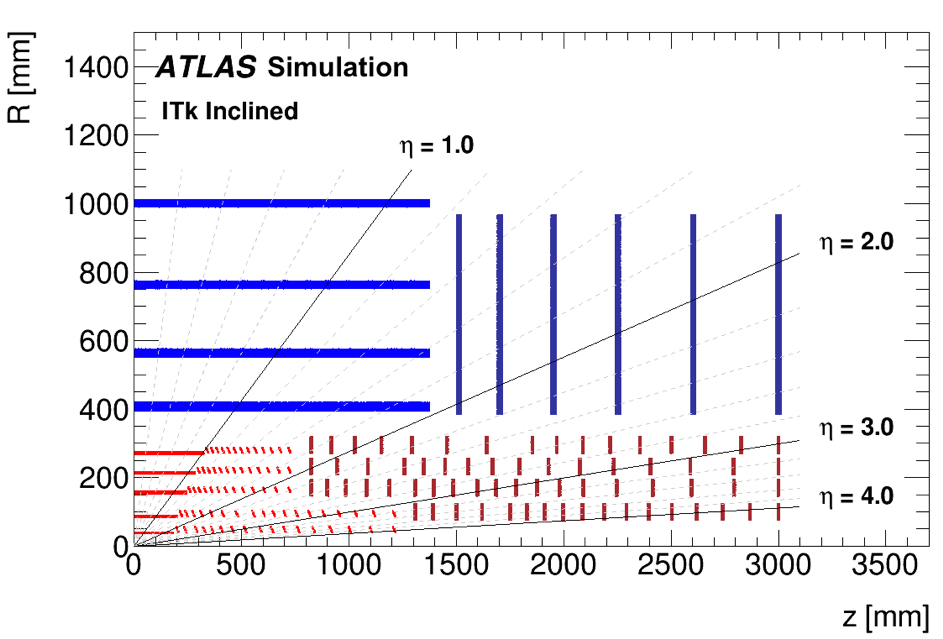
\includegraphics[width=11cm,height=8cm,keepaspectratio]{Figures/modules/Appendix/layout2.png}
    \caption{The Layout of the ITk Strip Detector. The left figure showcases the layout of the detector consisting of $4$ barrel layers (horizontal lines) and $6$ end-cap disks on each side. the point $0$ is the interaction point, and the horizontal axis is the axis along the beam line. Both figures show the rapidity (pseudorapidity) coverage of the ITk detector (red for ITk-Pixel and blue for ITk-Strip) with the barrel part covering $\eta \approx \pm 1.05$ and the total coverage of the detector is $\eta \approx \pm 2.7$\cite{Collaboration:390920} }
    \label{fig:additionalLayout}
\end{figure}

\newpage
\section{Barel and Enc-cap modules}
\begin{figure}[h]
    \begin{subfigure}[b]{1\textwidth}
        \centering
        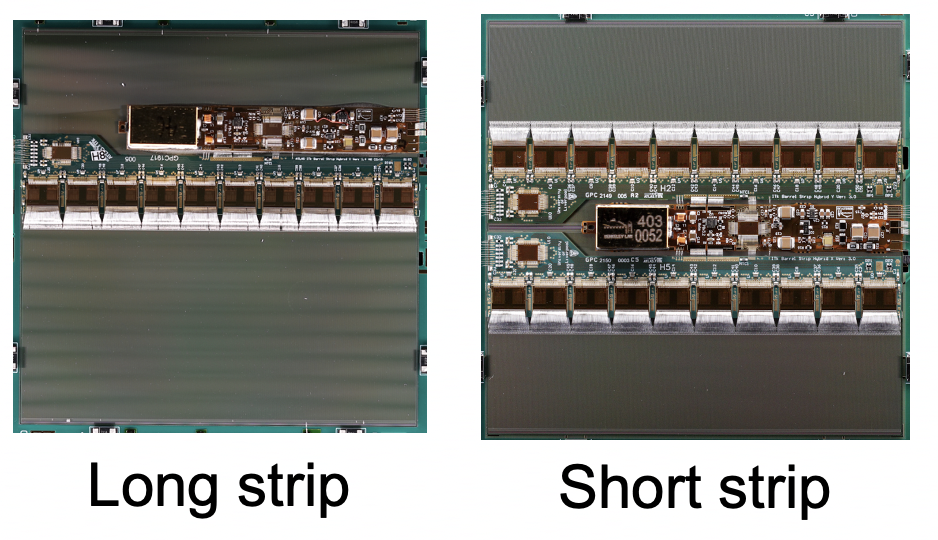
\includegraphics[width=14cm,height=15cm,keepaspectratio]{Figures/modules/Barrel_Modules.png}
        \caption{}\label{fig:barrel}
    \end{subfigure}
    \\
    \begin{subfigure}[b]{1\textwidth}
        \centering
        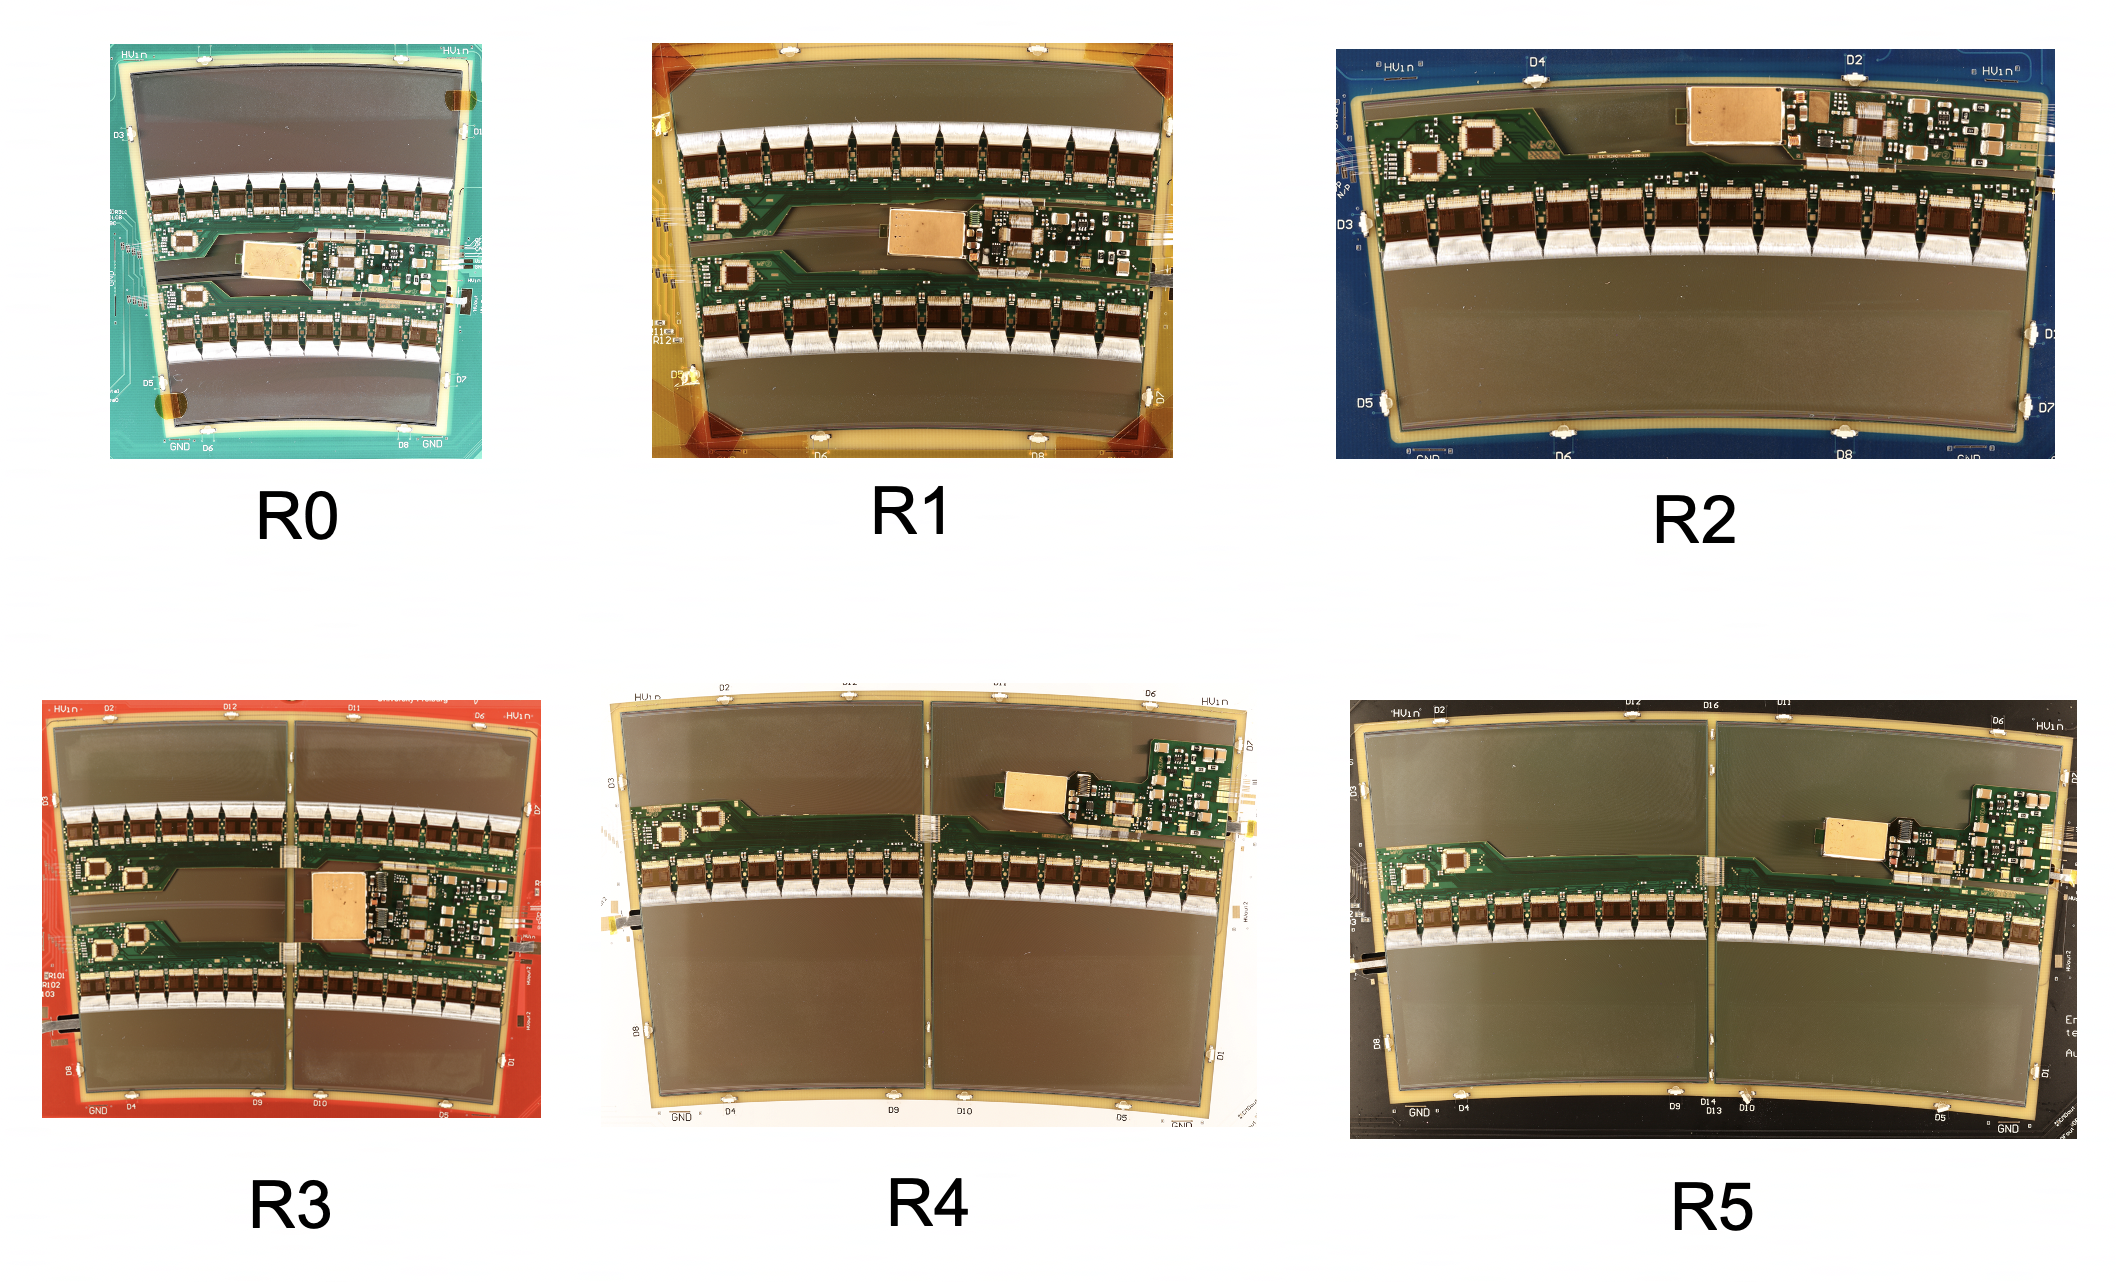
\includegraphics[width=14cm,height=15cm,keepaspectratio]{Figures/modules/EC_Modules.png}
        \caption{}\label{fig:endcap}
    \end{subfigure}
        \caption{Top view pictures of a) barrel modules including LS and SS, and b) end-cap modules including R0 to R5\cite{tishelman2024quality} }
        \label{fig:picModules-large}
\end{figure}

\newpage
\section{Coldbox}
\subsection{Power supllies}
\begin{figure}[h]
    \centering
    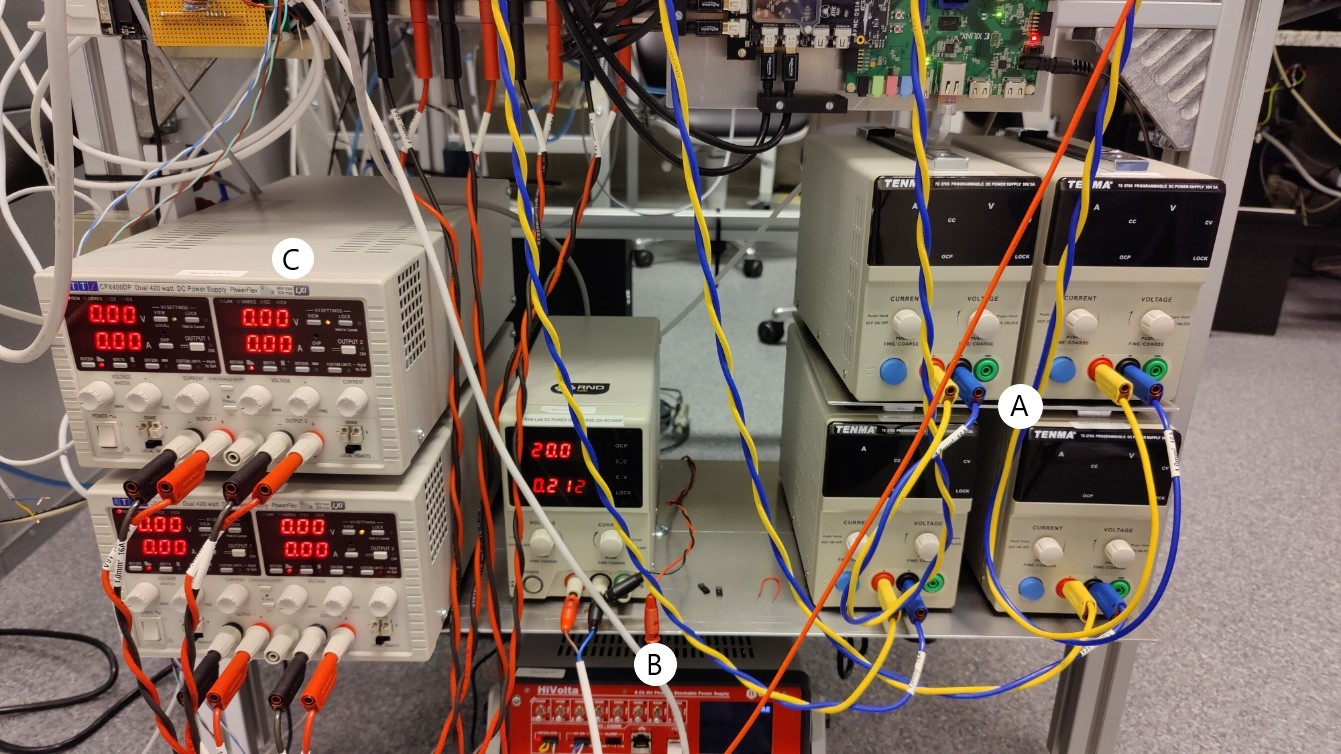
\includegraphics[width=14cm,height=11cm,keepaspectratio]{Figures/test/p-supplies.jpg}
    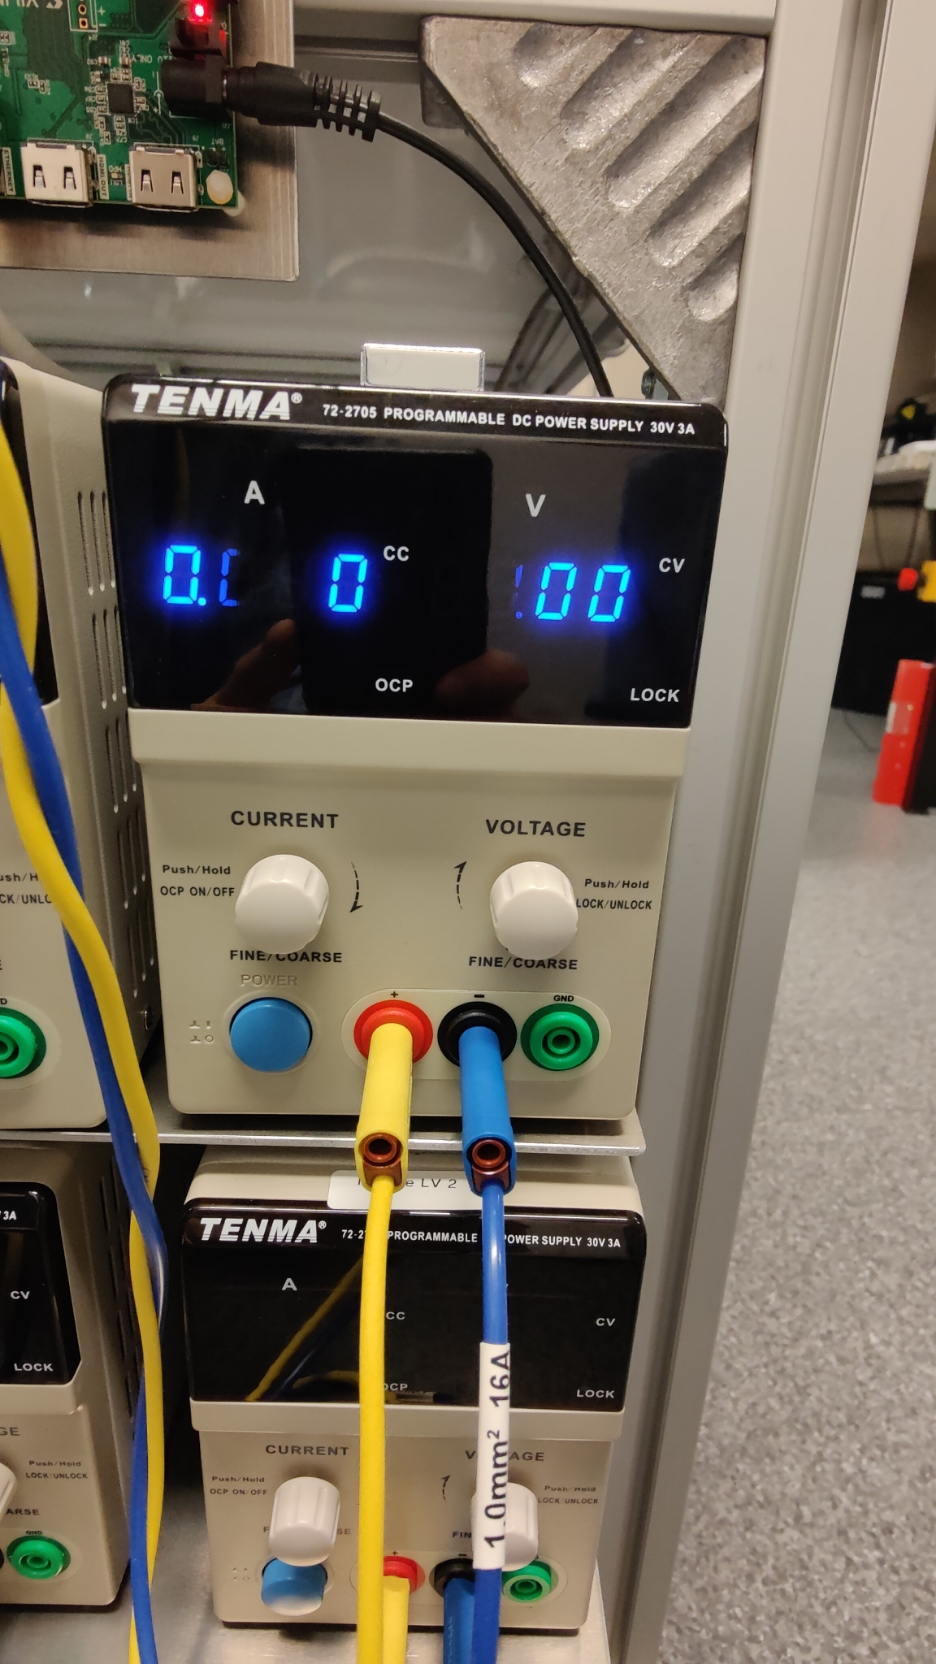
\includegraphics[width=7cm,height=7cm,keepaspectratio]{Figures/test/LV.jpg}
    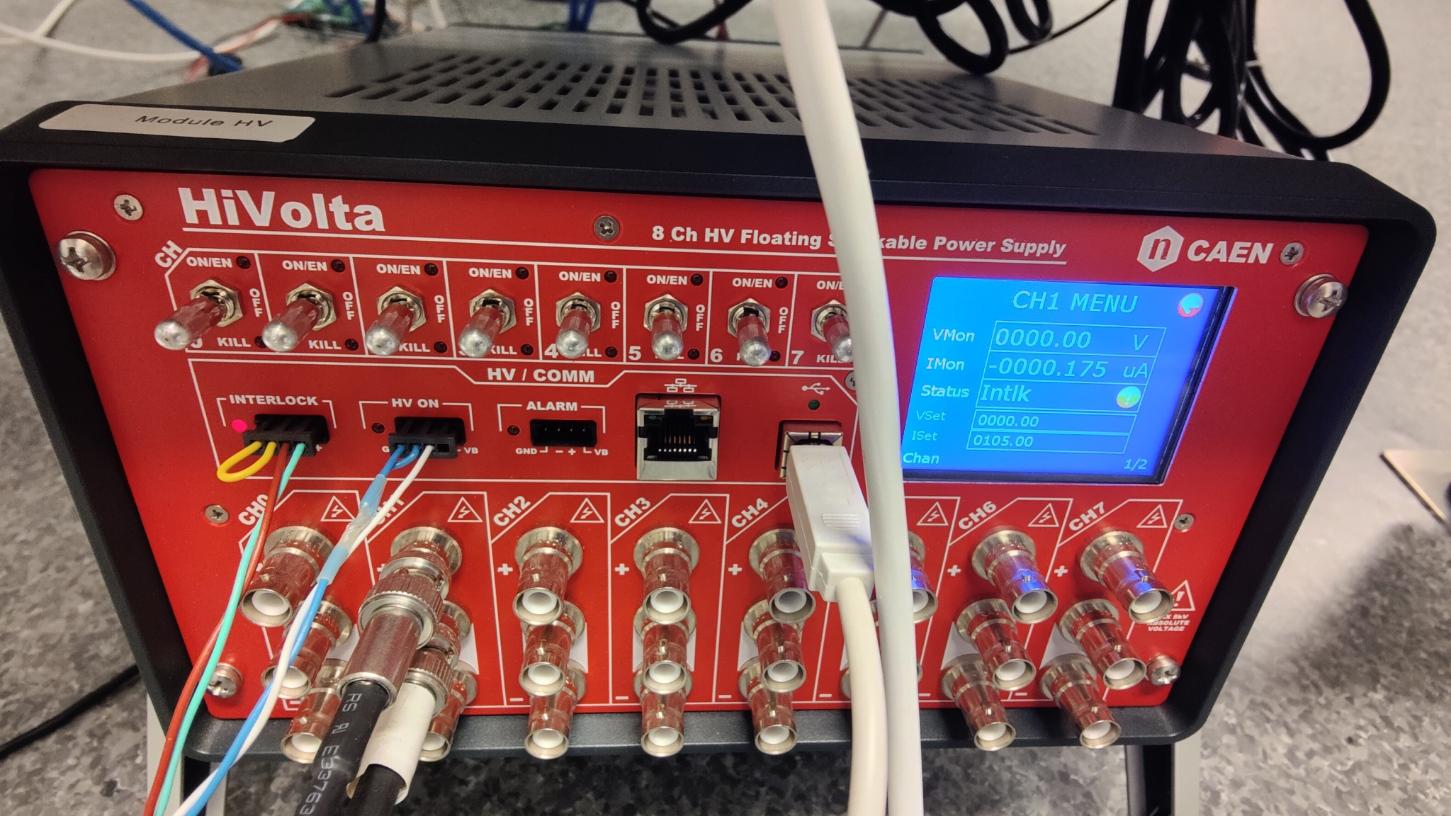
\includegraphics[width=10cm,height=10cm,keepaspectratio]{Figures/test/HV.jpg}
    
    \caption{Pictures of the power supplies: a) Low Voltage used to power the modules, b) High Voltage power supply to inject the test charge, and c) Peltier power supplies}
    \label{fig:supplies}
\end{figure}
\newpage
\subsection{Temperature and air flow}
\begin{figure}[h]
    \centering
    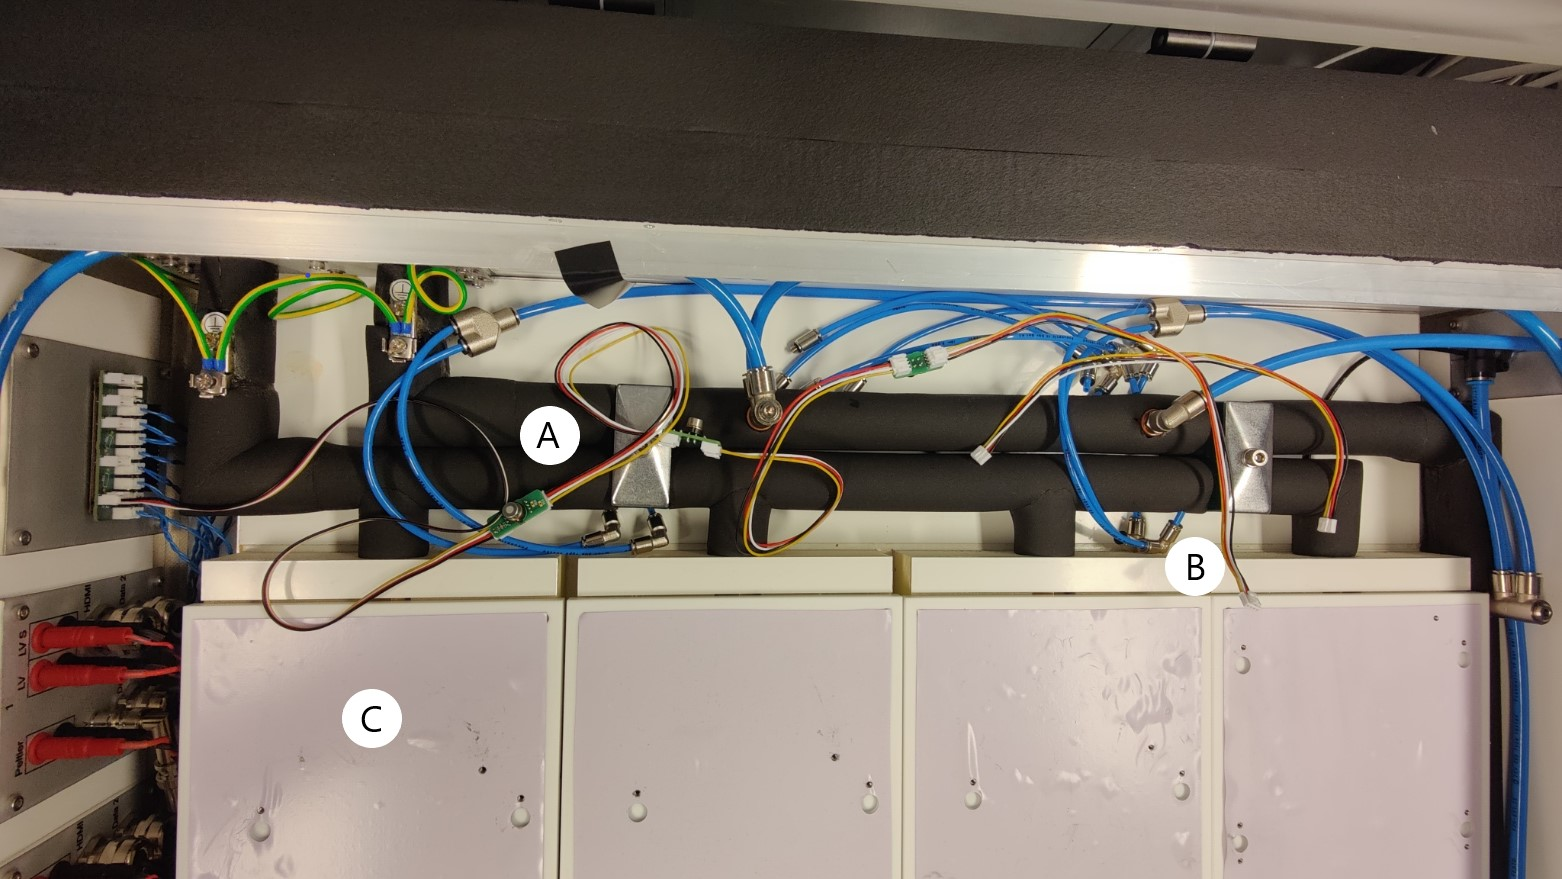
\includegraphics[width=10cm,height=11cm,keepaspectratio]{Figures/test/connections-2.jpg}
    \caption{An overview of the chiller and airflow connections showing a) chiller connections to each chuck using thermally isolated copper pipes, b) airflow connections, and c) Peltiers.}
    \label{fig:cooling}
\end{figure}
\begin{figure}[h]
    \begin{subfigure}[b]{0.45\textwidth}
        \centering
        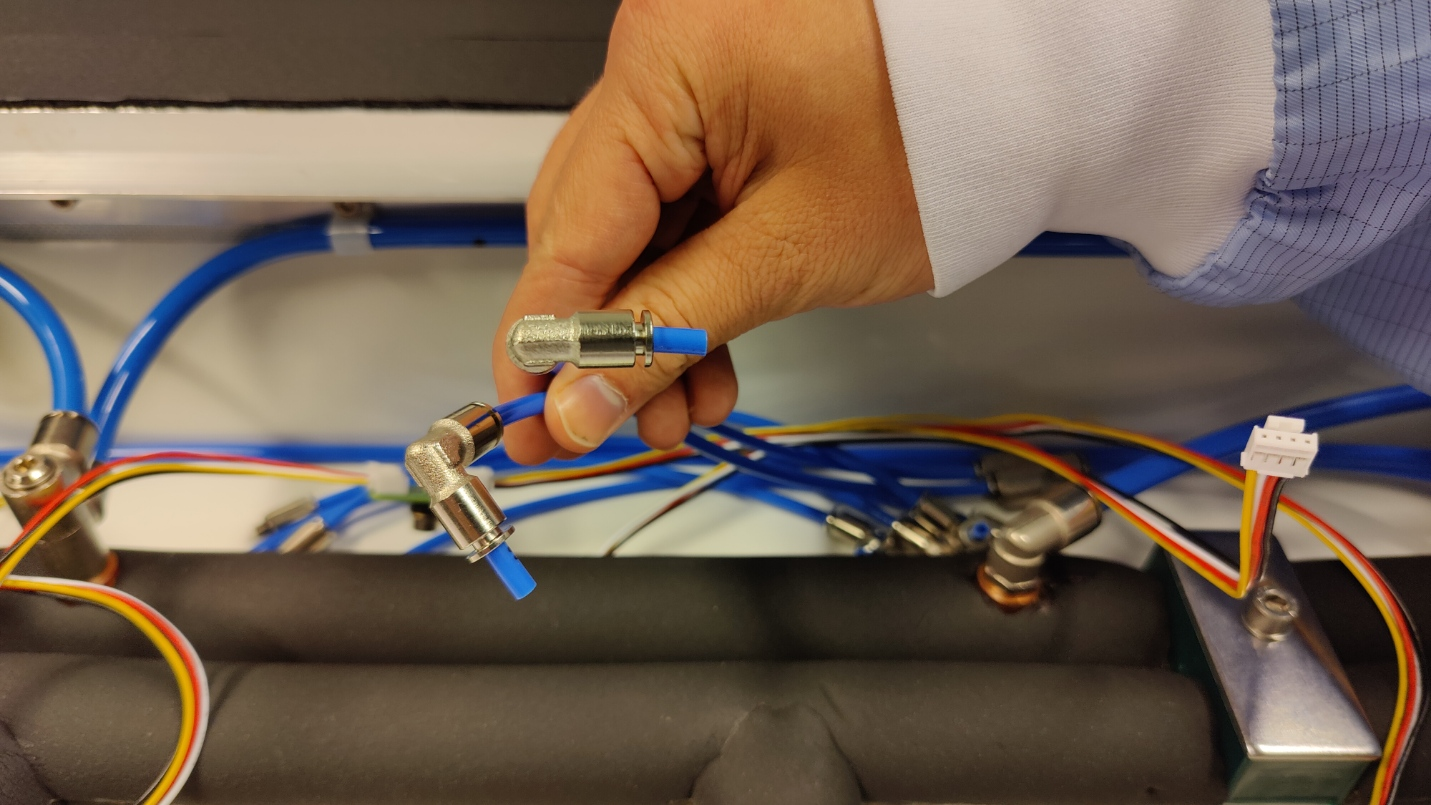
\includegraphics[width=7.5cm,height=10cm,keepaspectratio]{Figures/test/airflow-1.jpg}
        \caption{}\label{fig:airflow1}
    \end{subfigure}
    ~
    \begin{subfigure}[b]{0.45\textwidth}
        \centering
        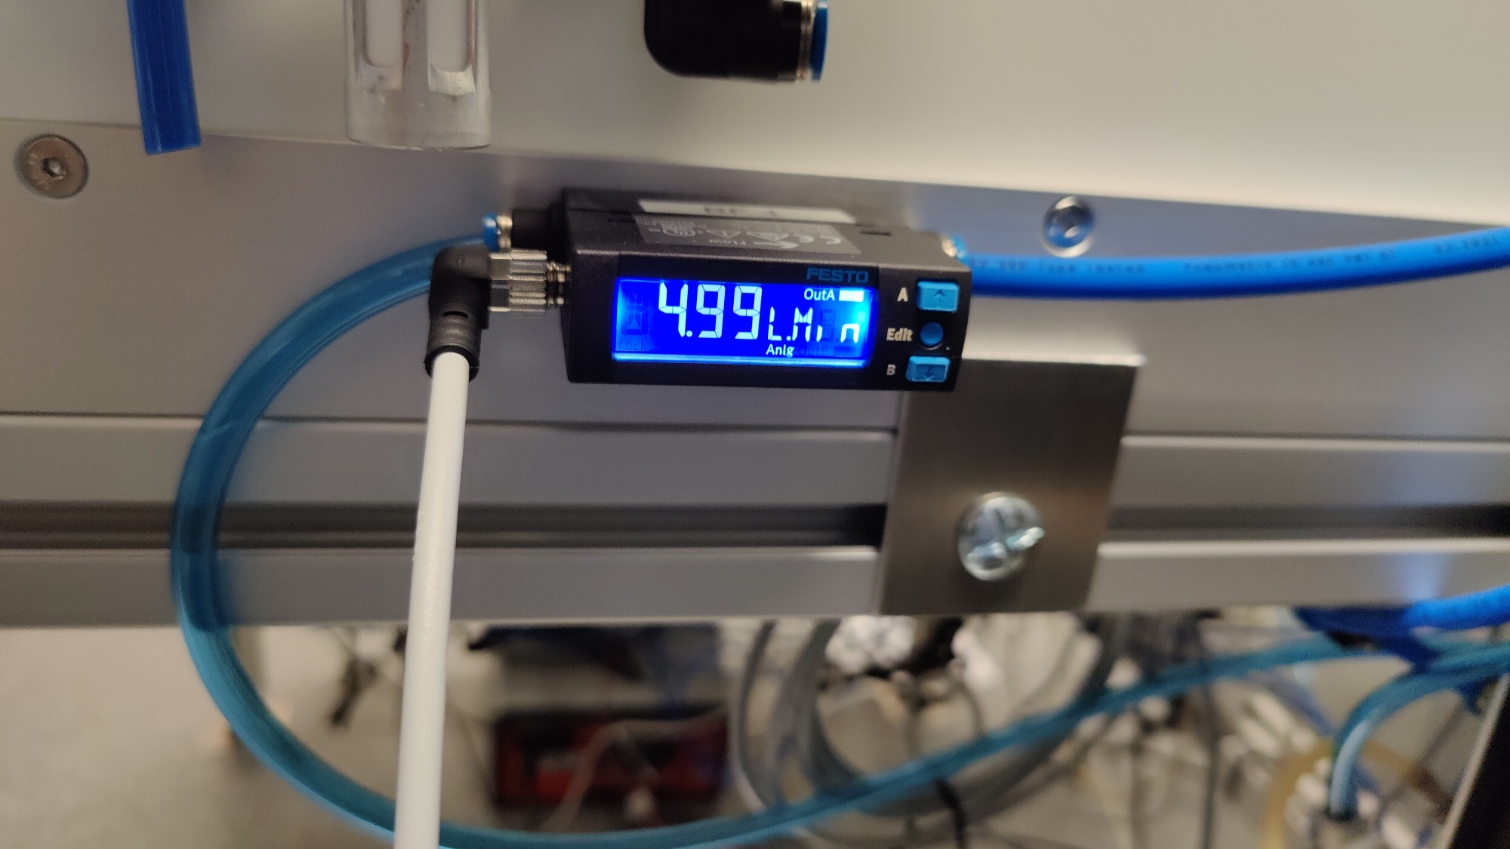
\includegraphics[width=7.5cm,height=10cm,keepaspectratio]{Figures/test/airflow-2.jpg}
        \caption{}\label{fig:airflow2}
    \end{subfigure}

    \begin{subfigure}[b]{0.45\textwidth}
        \centering
        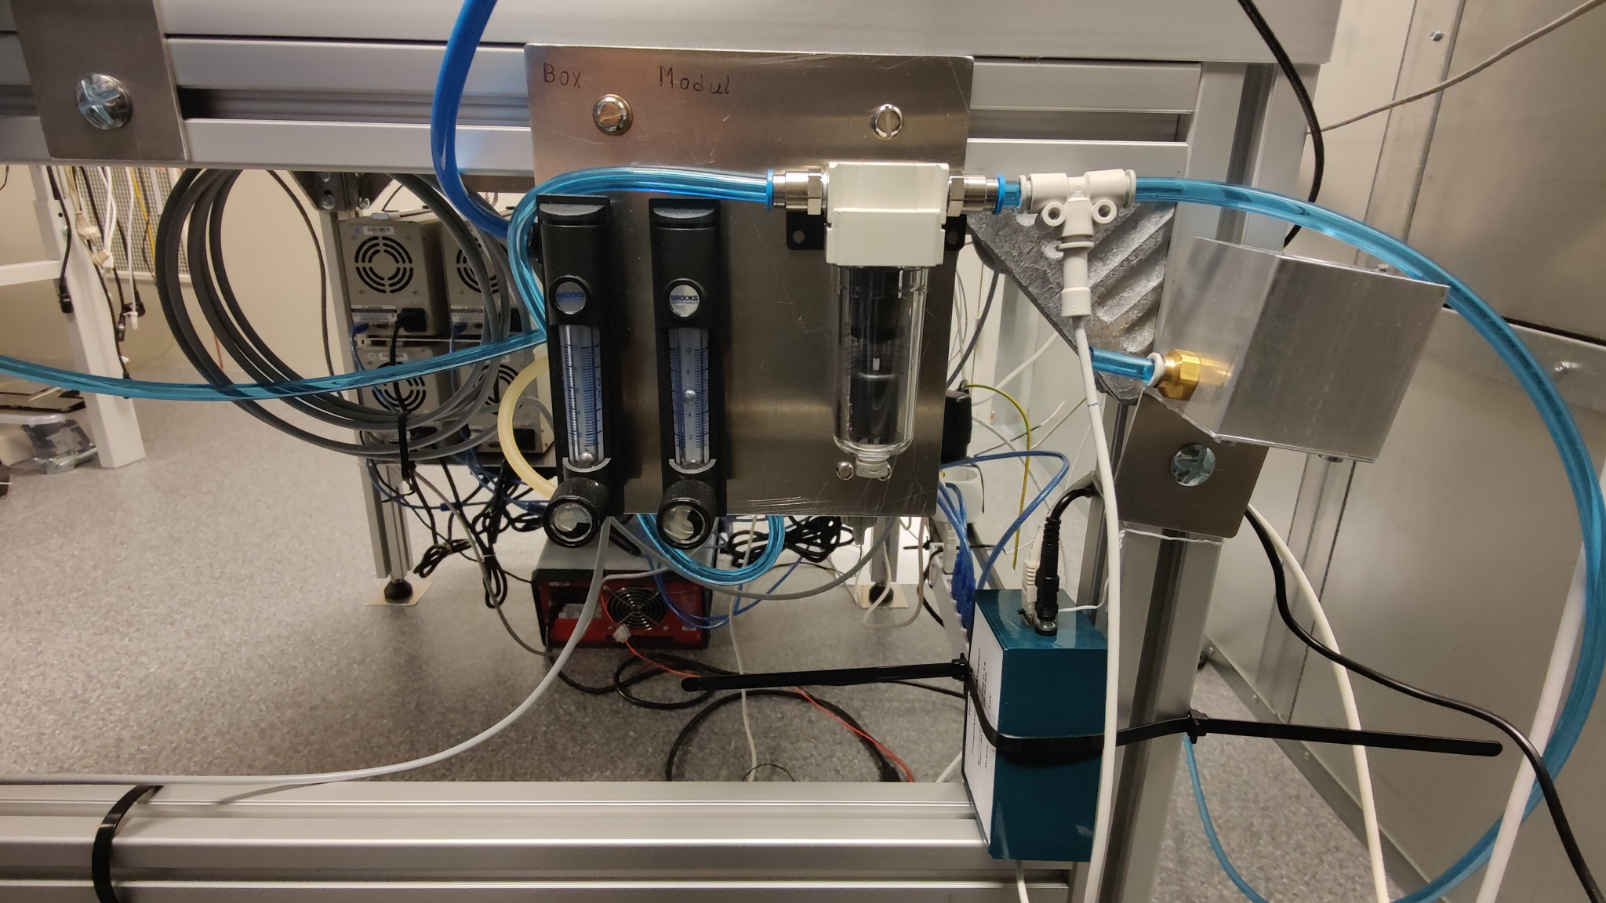
\includegraphics[width=7.5cm,height=10cm,keepaspectratio]{Figures/test/airflow-3.jpg}
        \caption{}\label{fig:airflow3}
    \end{subfigure}
    \caption{Picture of a) the airflow connectors, b) the Coldbox digital flowmeter, and c) flow control valves.}
    \label{fig:airflow}
\end{figure}

\newpage
\subsection{Electronics and connections}
\begin{figure}[h]
    \centering
    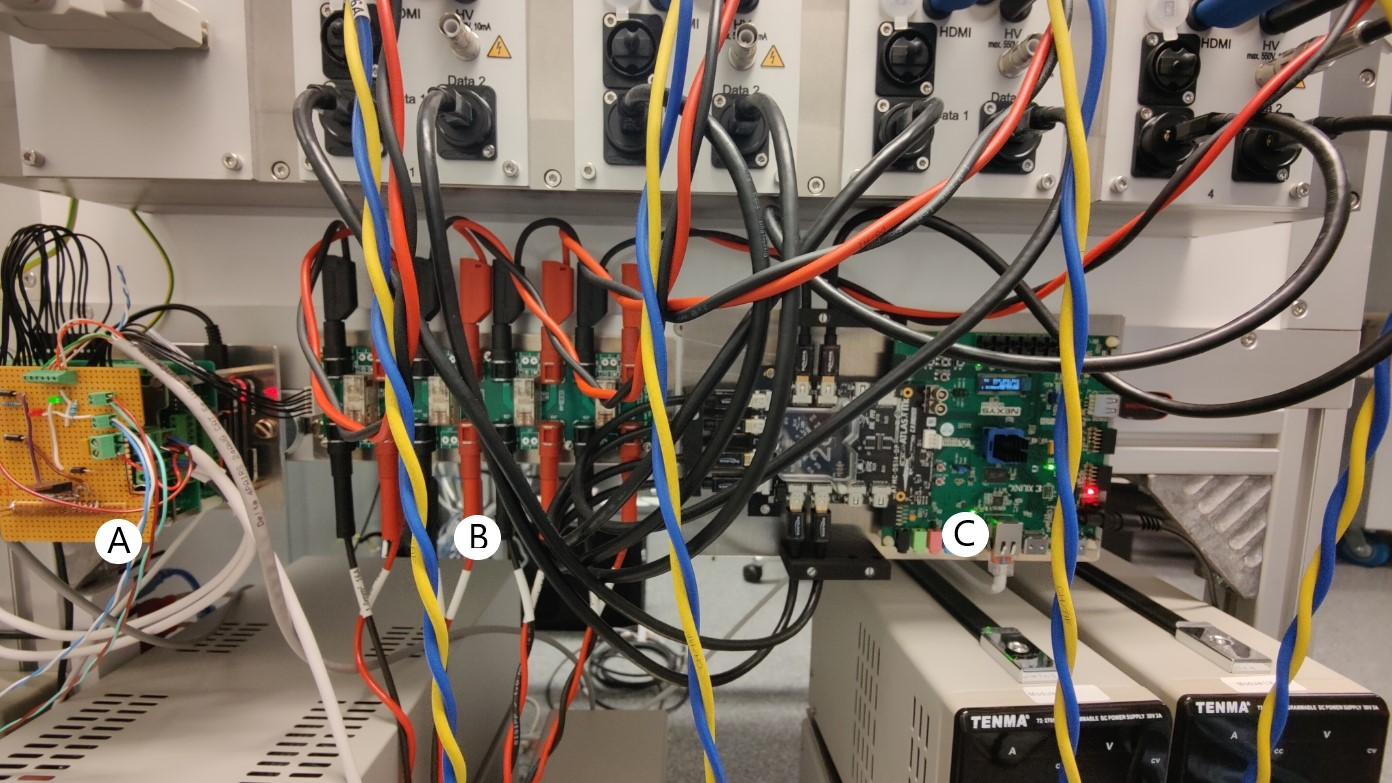
\includegraphics[width=10cm,height=11cm,keepaspectratio]{Figures/test/connections-5.jpg}
    \caption{An overview of the electronic and digital controllers and connections showing a) RPi (coldjiglib), b) Peltier switch and control board, and c) data ports}
    \label{fig:connections}
\end{figure}

\begin{figure}[h]
    
    \begin{subfigure}[b]{0.45\textwidth}
        \centering
        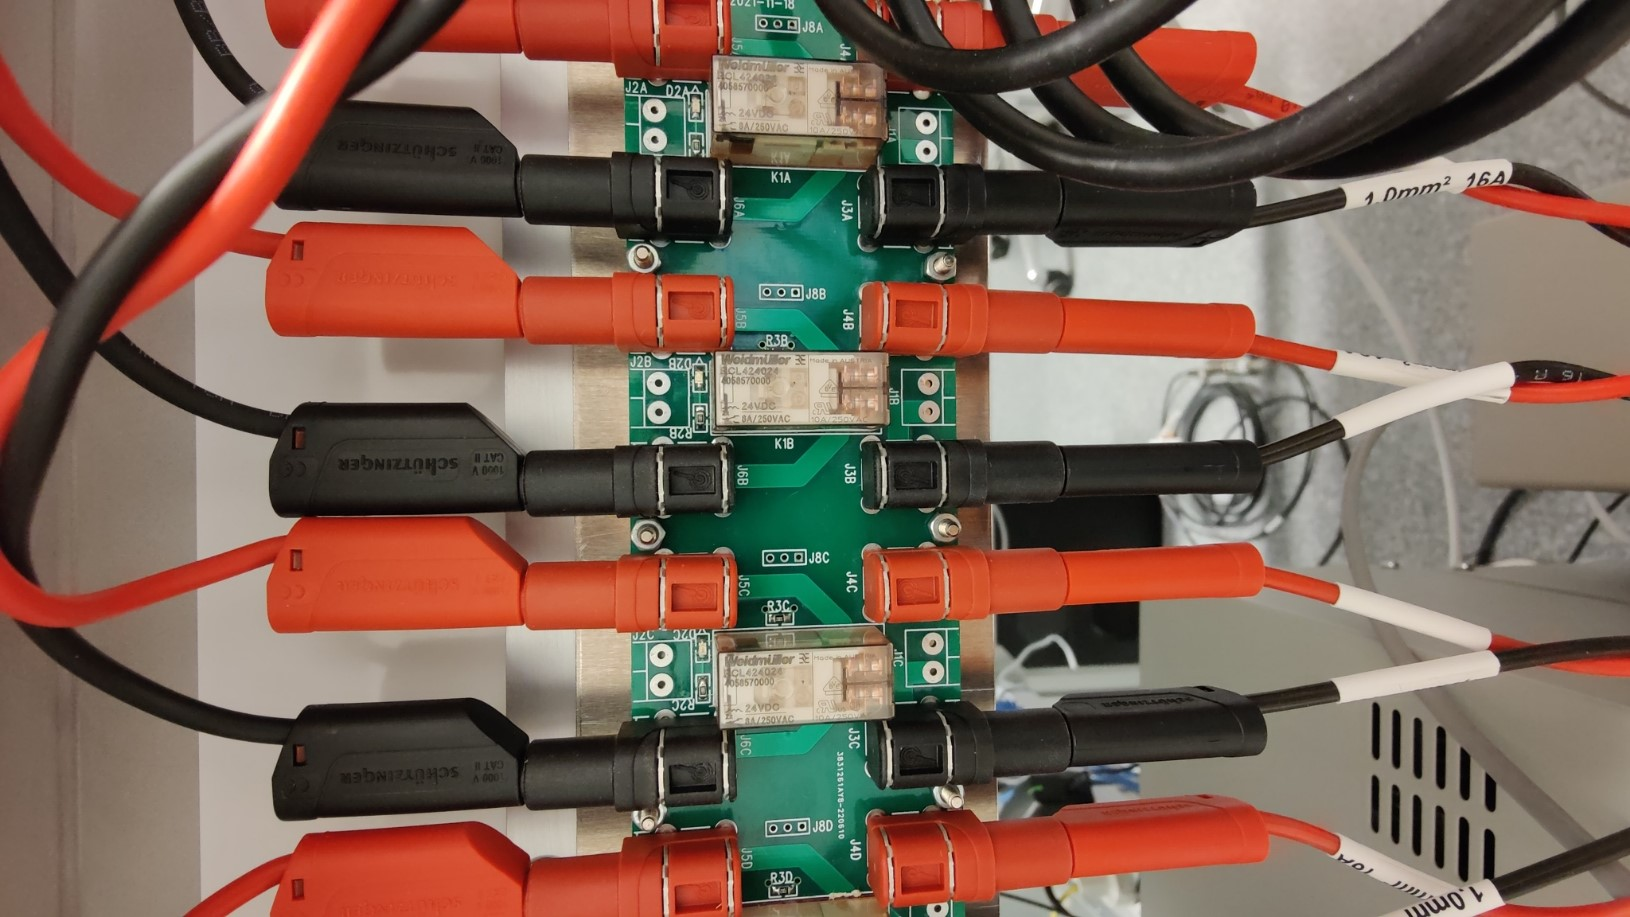
\includegraphics[width=7cm,height=10cm,keepaspectratio]{Figures/test/connections-3.jpg}
        \caption{}\label{fig:peltier1}
    \end{subfigure}
    ~
    \begin{subfigure}[b]{0.45\textwidth}
        \centering
        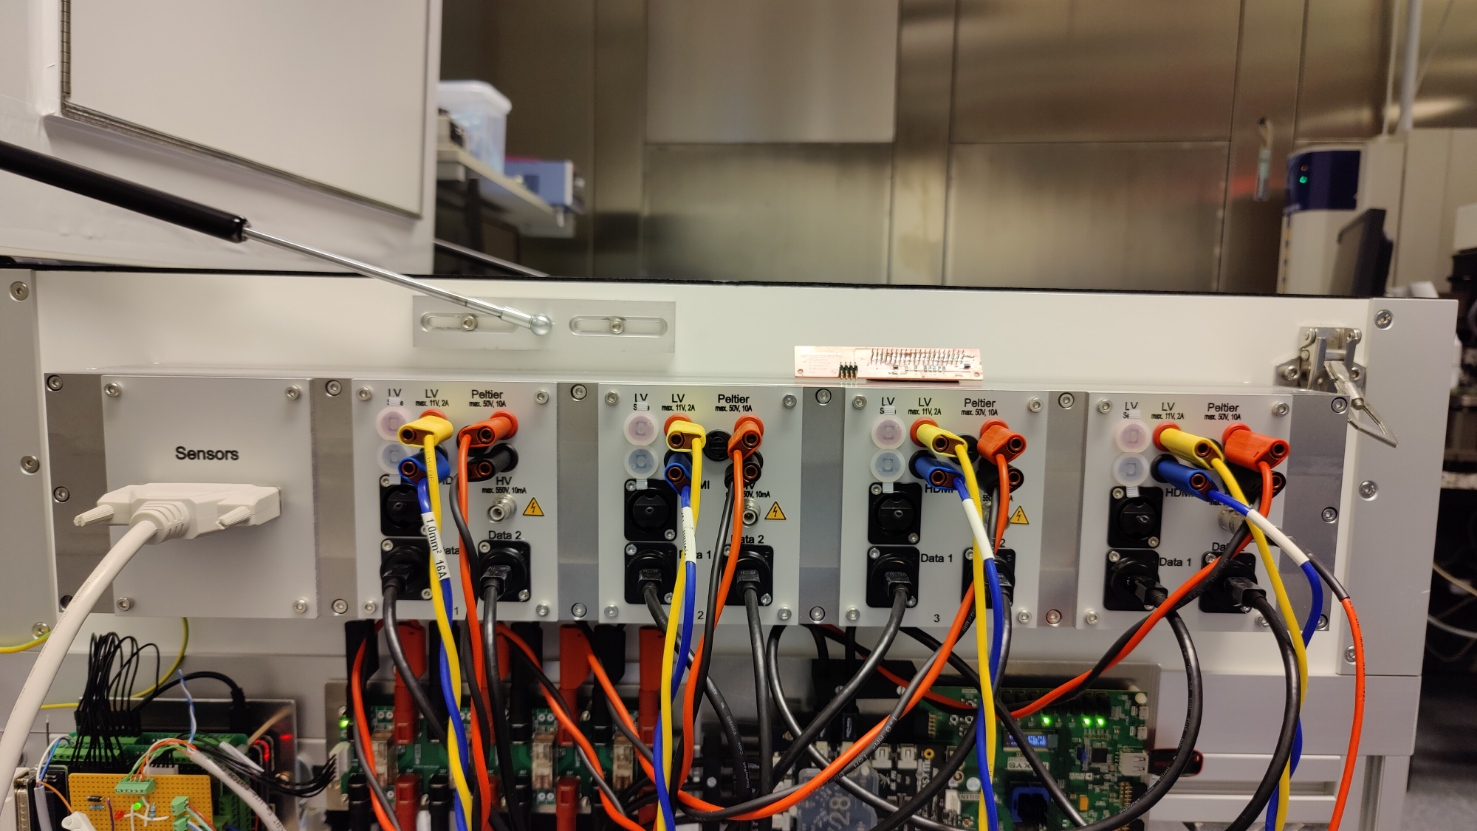
\includegraphics[width=7cm,height=10cm,keepaspectratio]{Figures/test/connections-6.jpg}
        \caption{}\label{fig:peltier2}
    \end{subfigure}

    \begin{subfigure}[b]{0.45\textwidth}
        \centering
        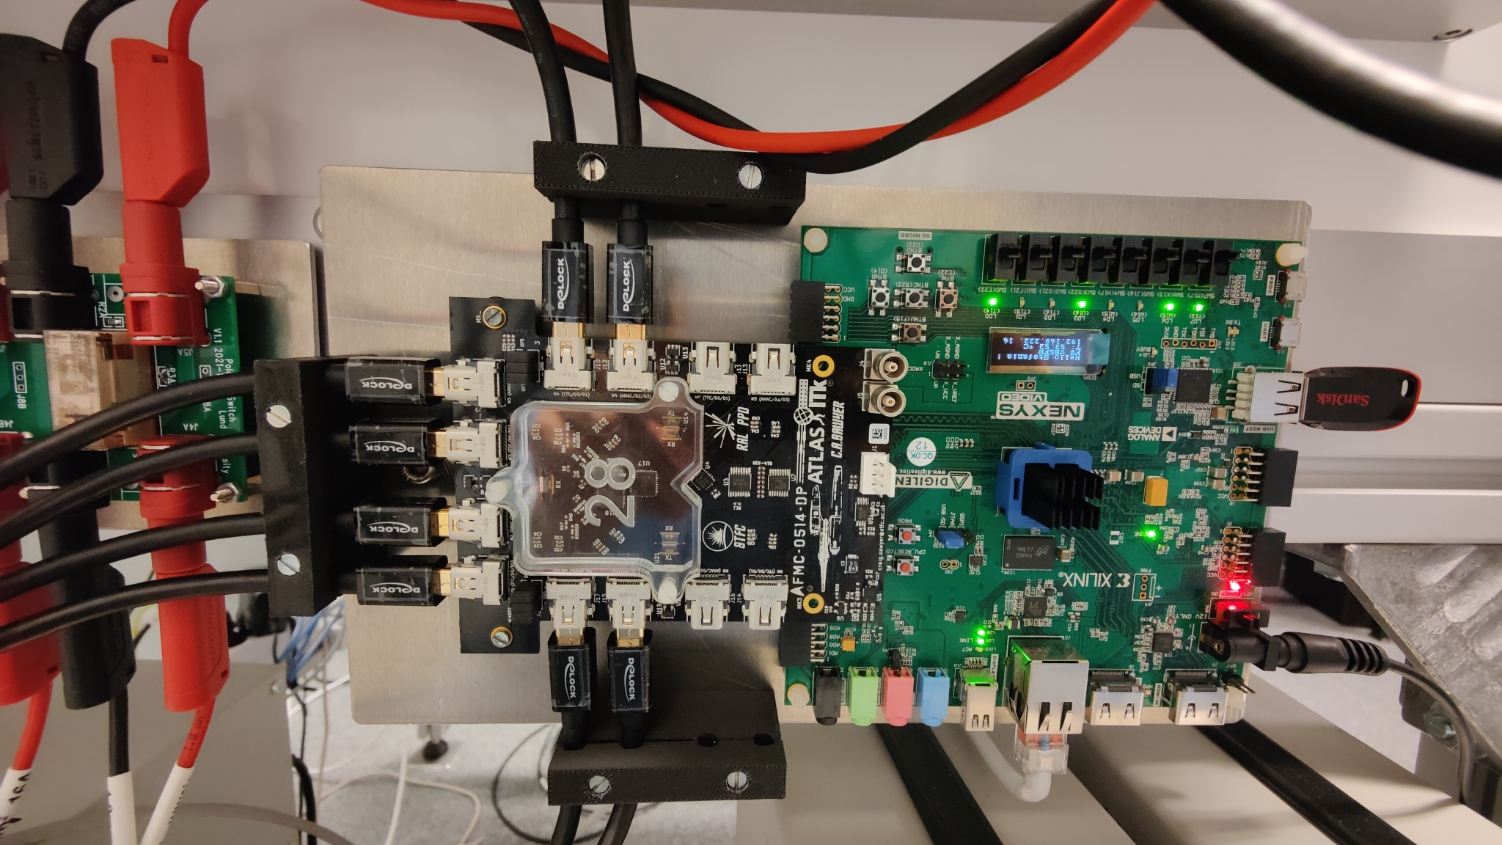
\includegraphics[width=7cm,height=10cm,keepaspectratio]{Figures/test/connections-4.jpg}
        \caption{}\label{fig:data}
    \end{subfigure}
    \caption{Picture of a) Peltier switchboard and controls, b) Peltier power connections, and c) data ports board}
    \label{fig:boards}
\end{figure}

\newpage
\subsection{Interlock}
\begin{figure}[h]
    \centering
    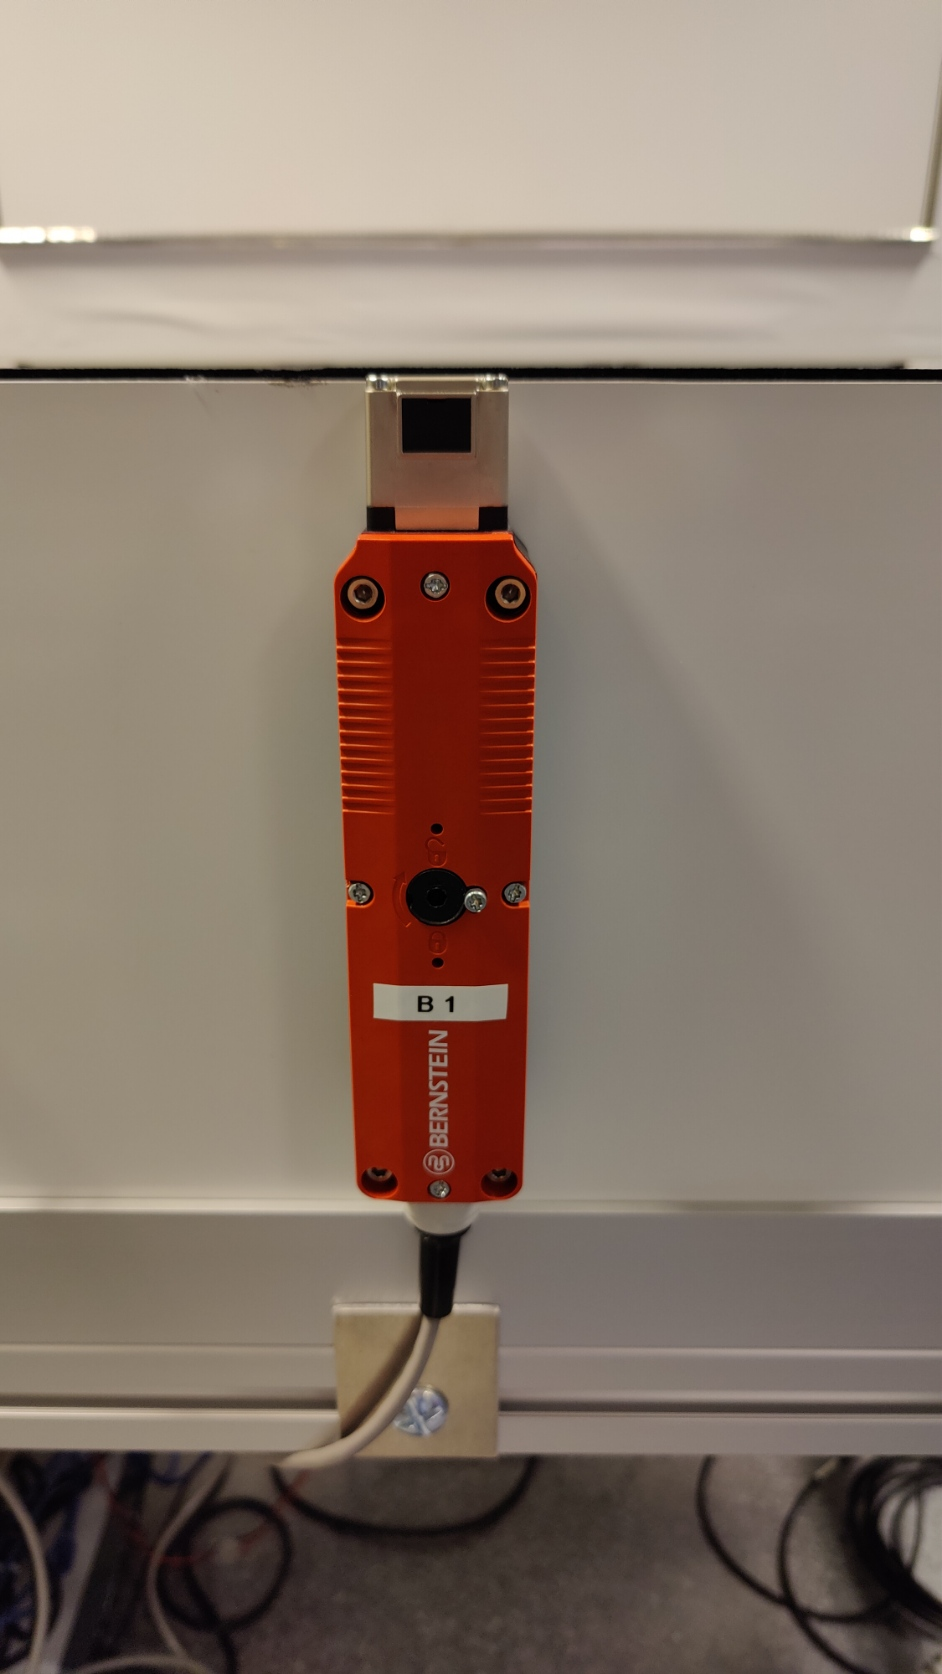
\includegraphics[width=10cm,height=11cm,keepaspectratio]{Figures/test/interlock.jpg}
    \caption{Picture of installed Interlock system on the Coldbox}
    \label{fig:interlock}
\end{figure}

\newpage
\subsection{Installation of modules}
\begin{figure}[h]    
    \begin{subfigure}[b]{0.4\textwidth}
        \centering
        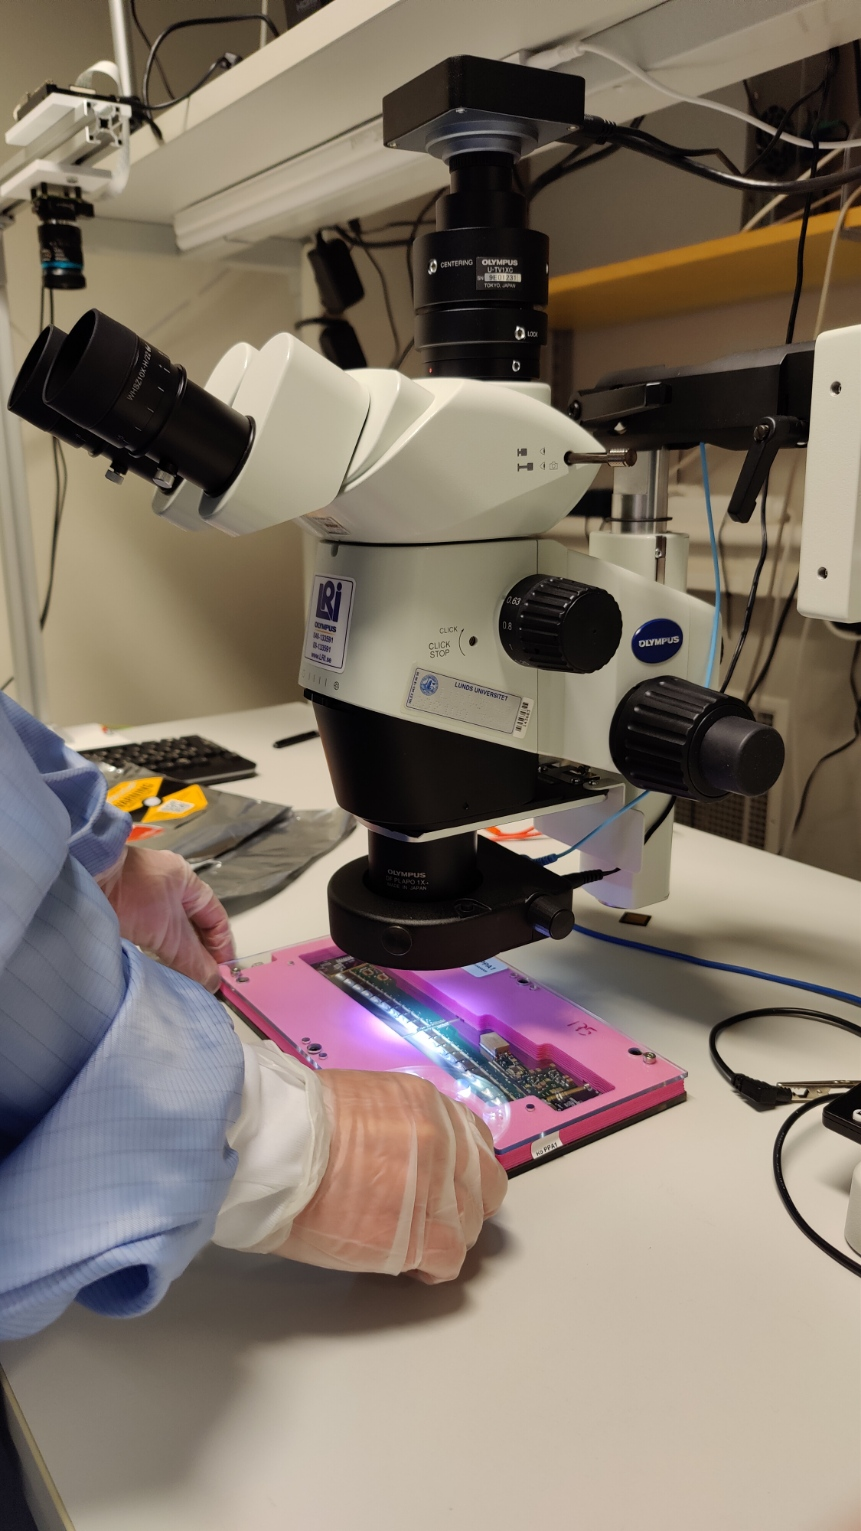
\includegraphics[width=7cm,height=8.5cm,keepaspectratio]{Figures/test/installation-4.jpg}
        \caption{}\label{fig:peltier1}
    \end{subfigure}
    ~
    \begin{subfigure}[b]{0.4\textwidth}
        \centering
        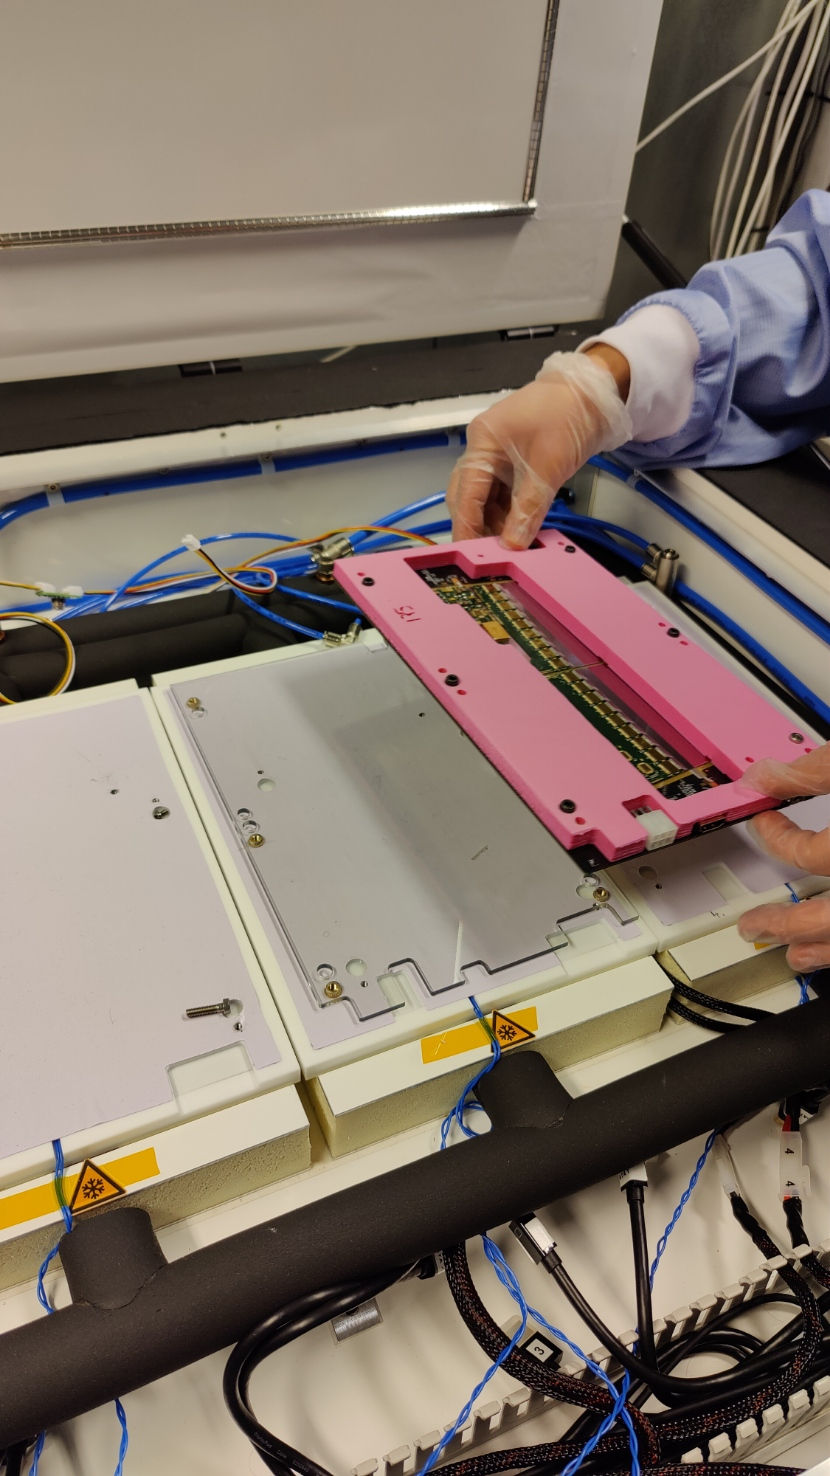
\includegraphics[width=7cm,height=8.5cm,keepaspectratio]{Figures/test/installation-2.jpg}
        \caption{}\label{fig:peltier2}
    \end{subfigure}

    \begin{subfigure}[b]{0.4\textwidth}
        \centering
        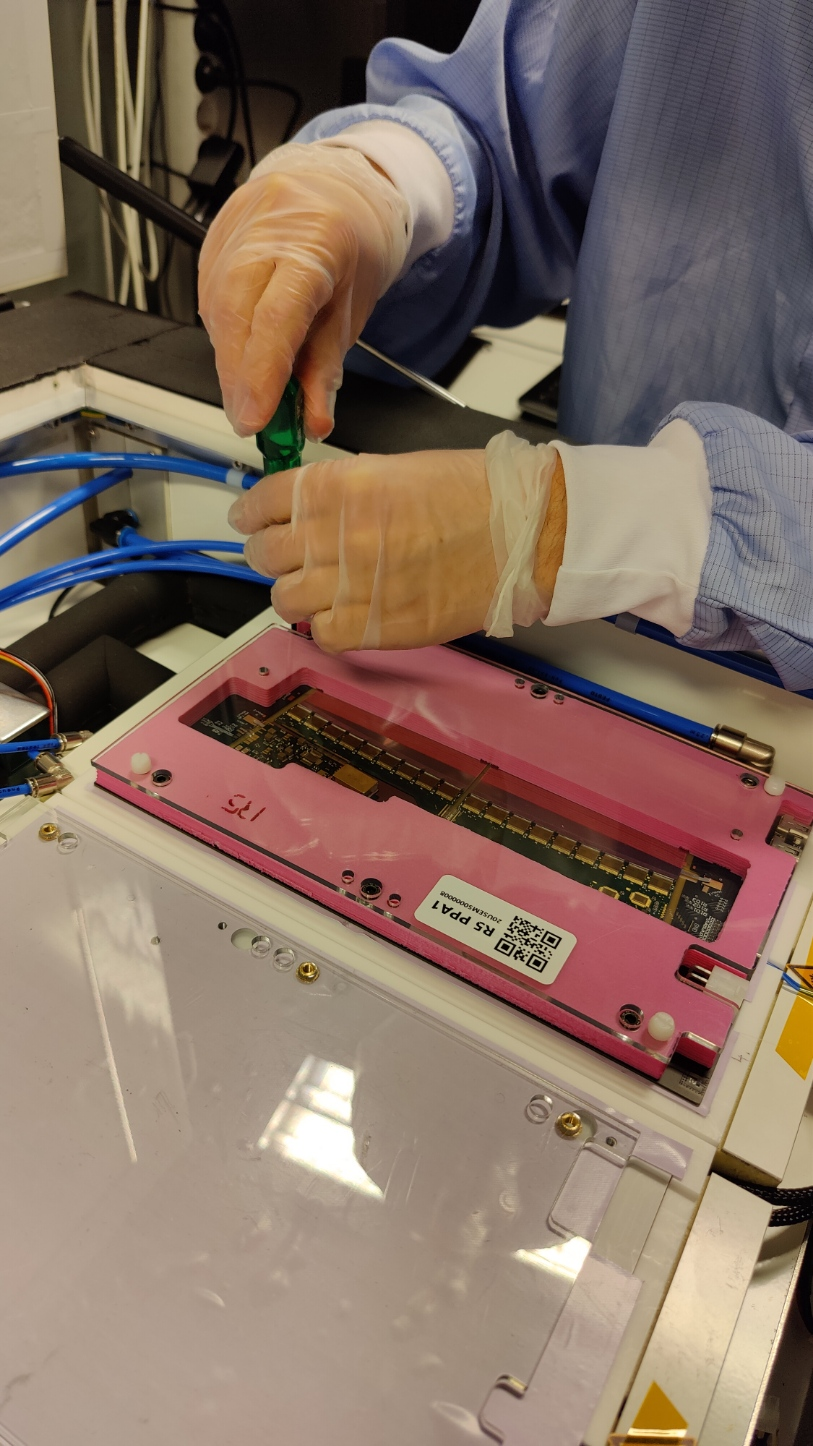
\includegraphics[width=7cm,height=8.5cm,keepaspectratio]{Figures/test/installation-1.jpg}
        \caption{}\label{fig:data}
    \end{subfigure}
    \caption{Inspection and installation of modules to the Coldbox}
    \label{fig:installation}
\end{figure}

\newpage
\section{Large format of Results' plots}

\begin{sidewaysfigure}[h]
    \centering
    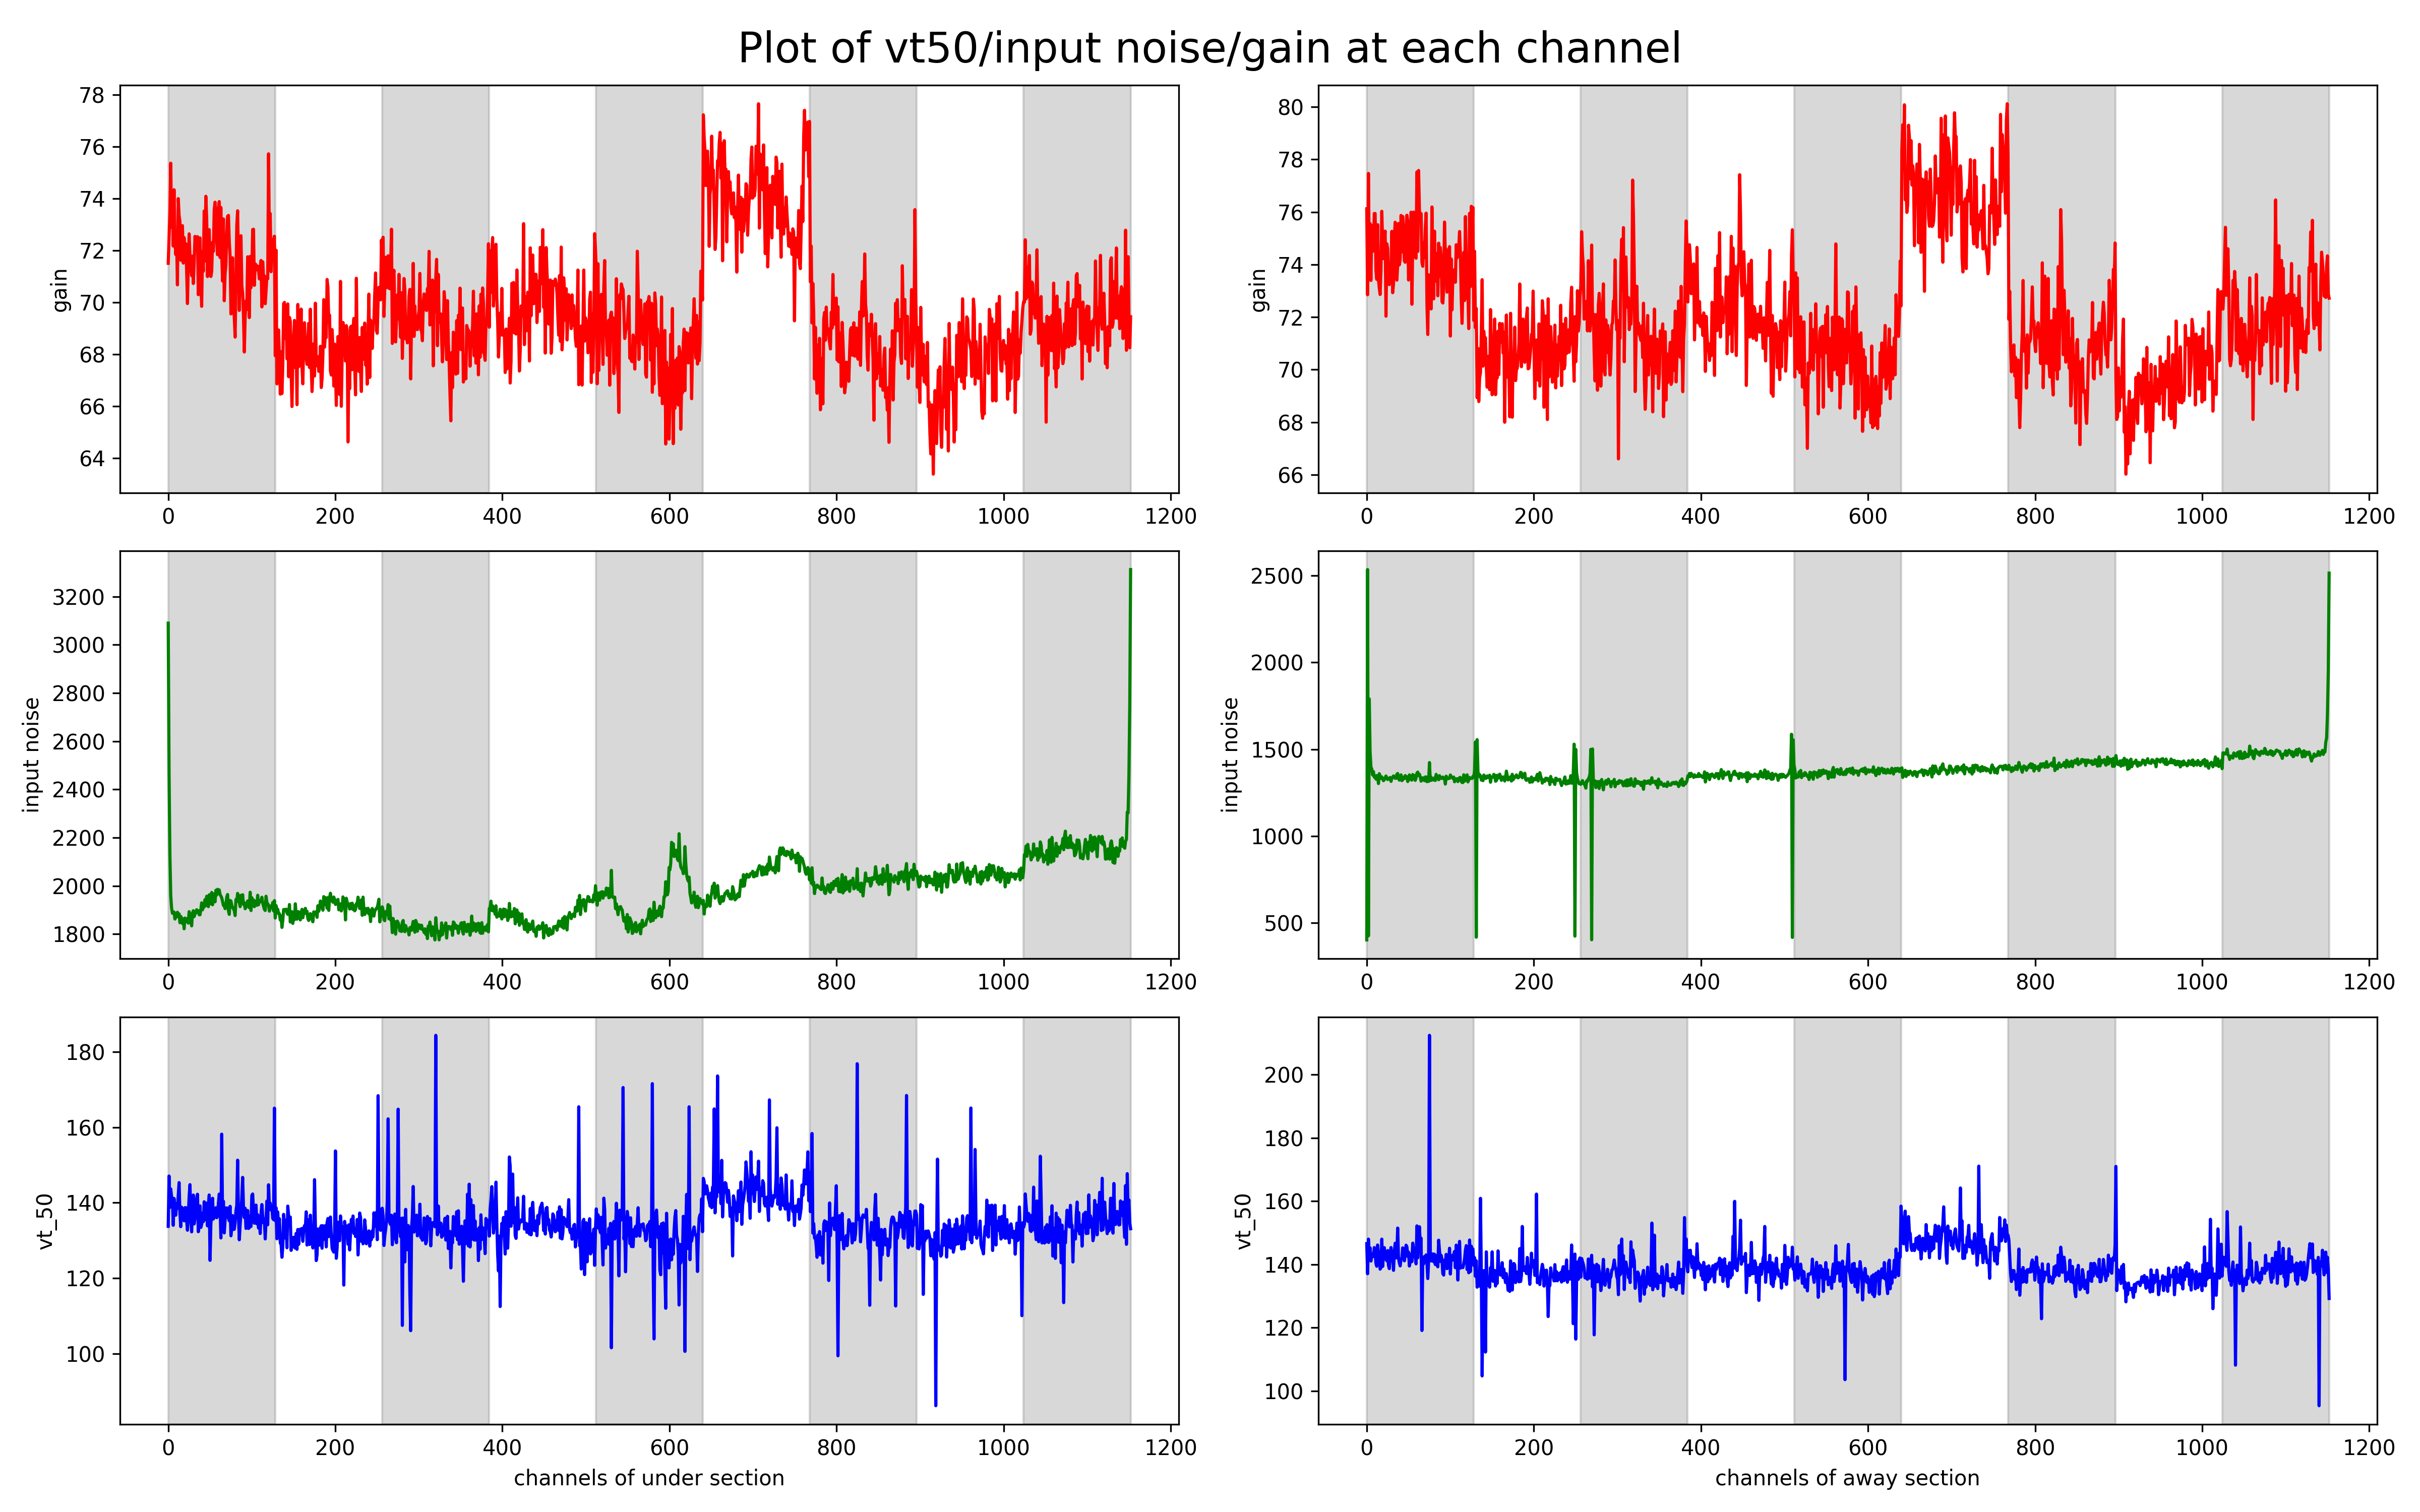
\includegraphics[width=25cm,height=20cm,keepaspectratio]{Figures/results/LTRT_1_plot.png}
    \caption{Plots of $3$ performed electrical test by ABCstar full test during the "LTRT COLD TEST 1" stage, showing the result of VT$50$, input noise, and gain for two hybrids (under and above) of a Pre Production A (PPA) R5 module.}
    \label{fig:LTRT_result_1_large}
\end{sidewaysfigure}

\begin{sidewaysfigure}[h]
    \centering
    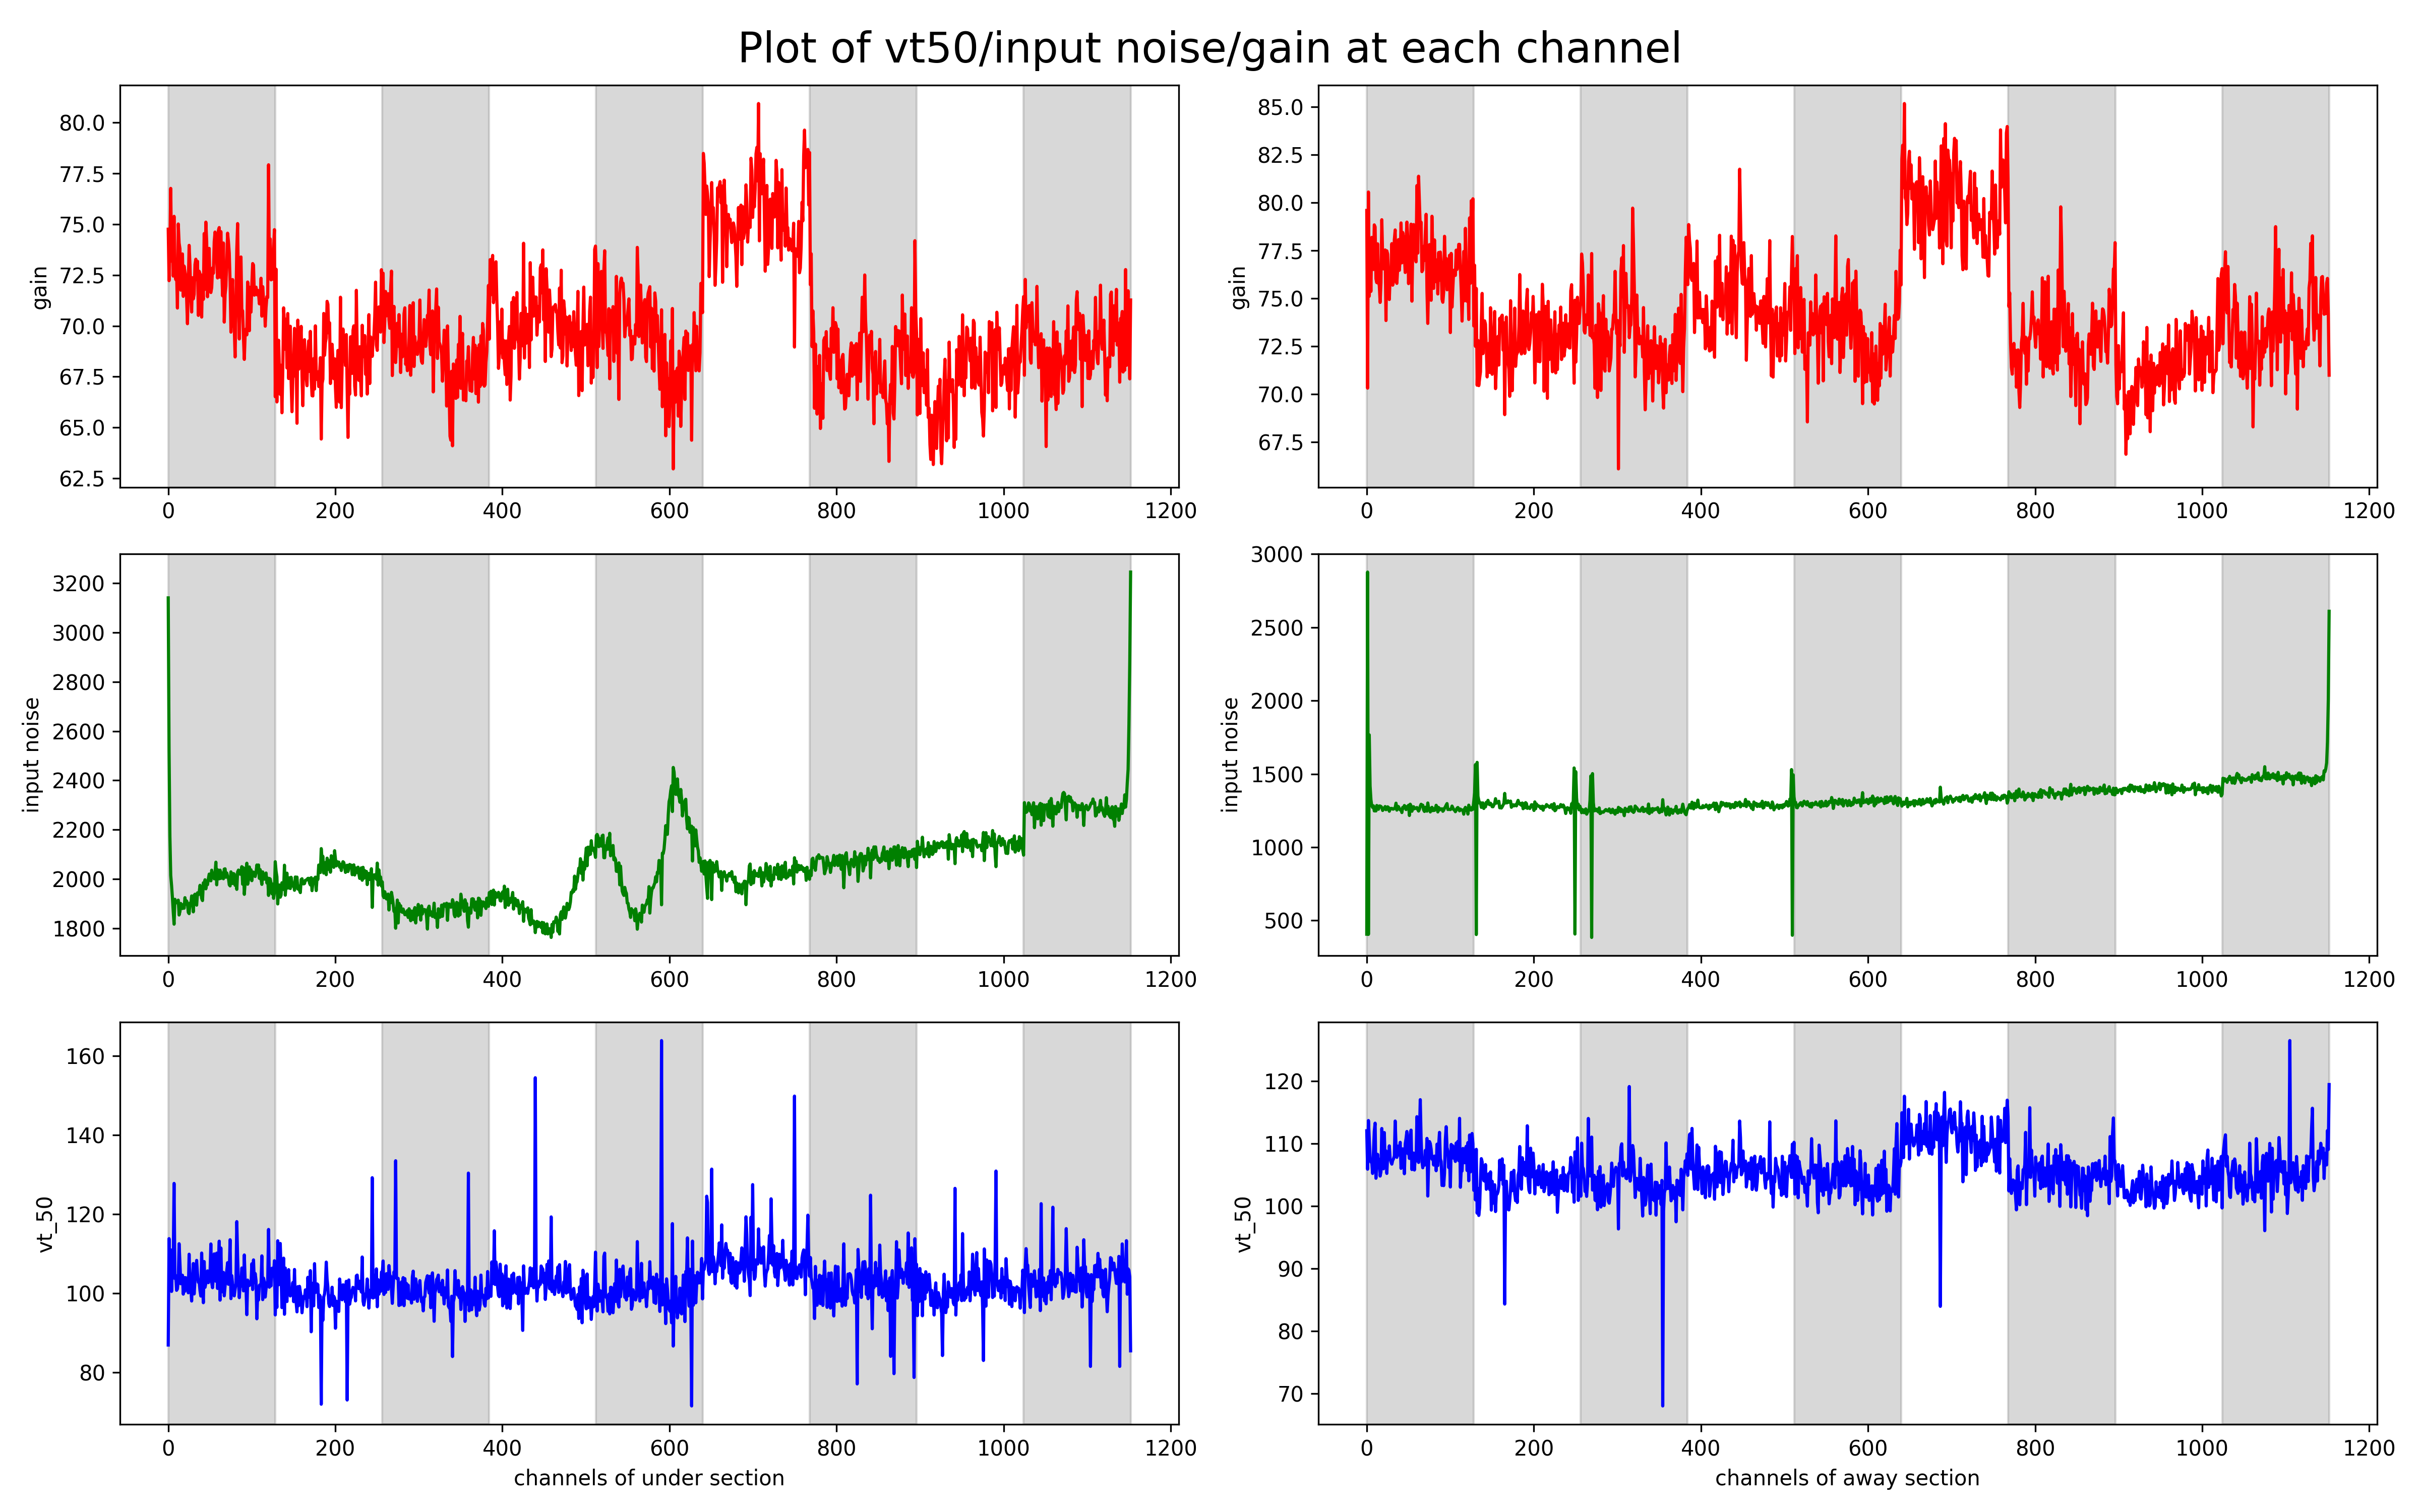
\includegraphics[width=25cm,height=20cm,keepaspectratio]{Figures/results/LTRT_2_plot.png}
    \caption{Plots of $3$ performed electrical test by ABCstar full test during the "LTRT COLD TEST 2" stage, showing the result of VT$50$, input noise, and gain for two hybrids (under and above) of a Pre Production A (PPA) R5 module.}
    \label{fig:LTRT_result_2_large}
\end{sidewaysfigure}

\begin{sidewaysfigure}[h]
    \centering
    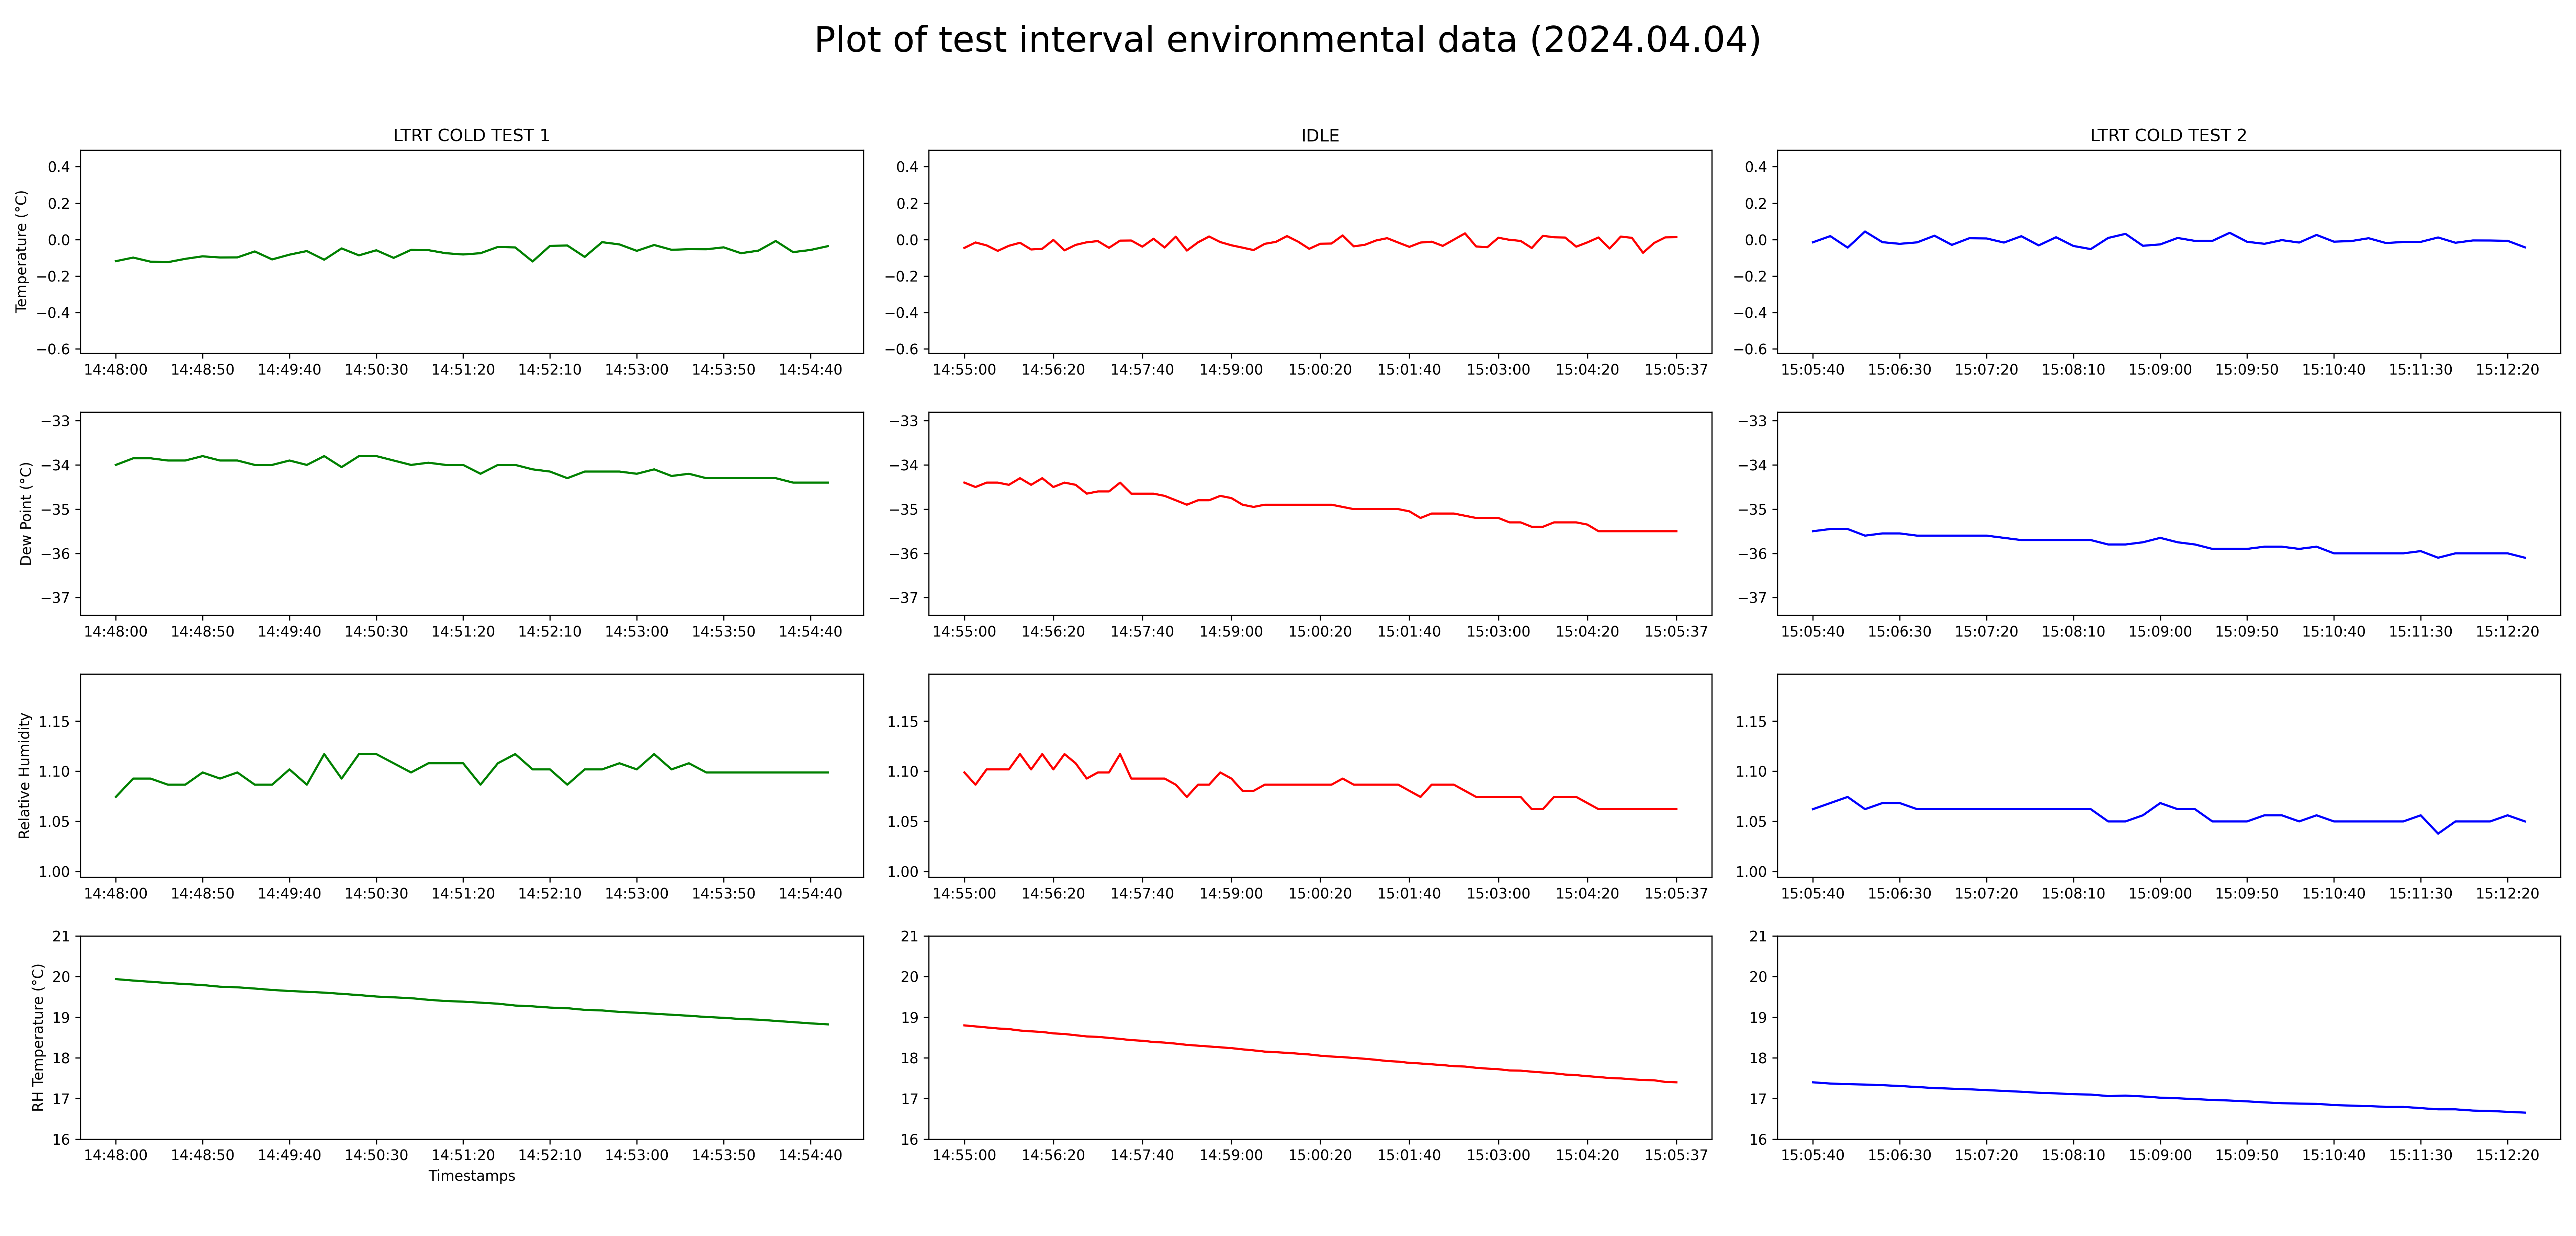
\includegraphics[width=25cm,height=20cm,keepaspectratio]{Figures/results/env_plot_20240404.png}
    \caption{Plots environmental data during the time span of the LTRT test shown in Fig.\ref{fig:LTRT_result_1_large} and Fig.\ref{fig:LTRT_result_2_large} showing the data for Temperature, Dew point, Relative humidity, and Relative humidity temperature.}
    \label{fig:env_1_large}
\end{sidewaysfigure}

\begin{sidewaysfigure}[h]
    \centering
    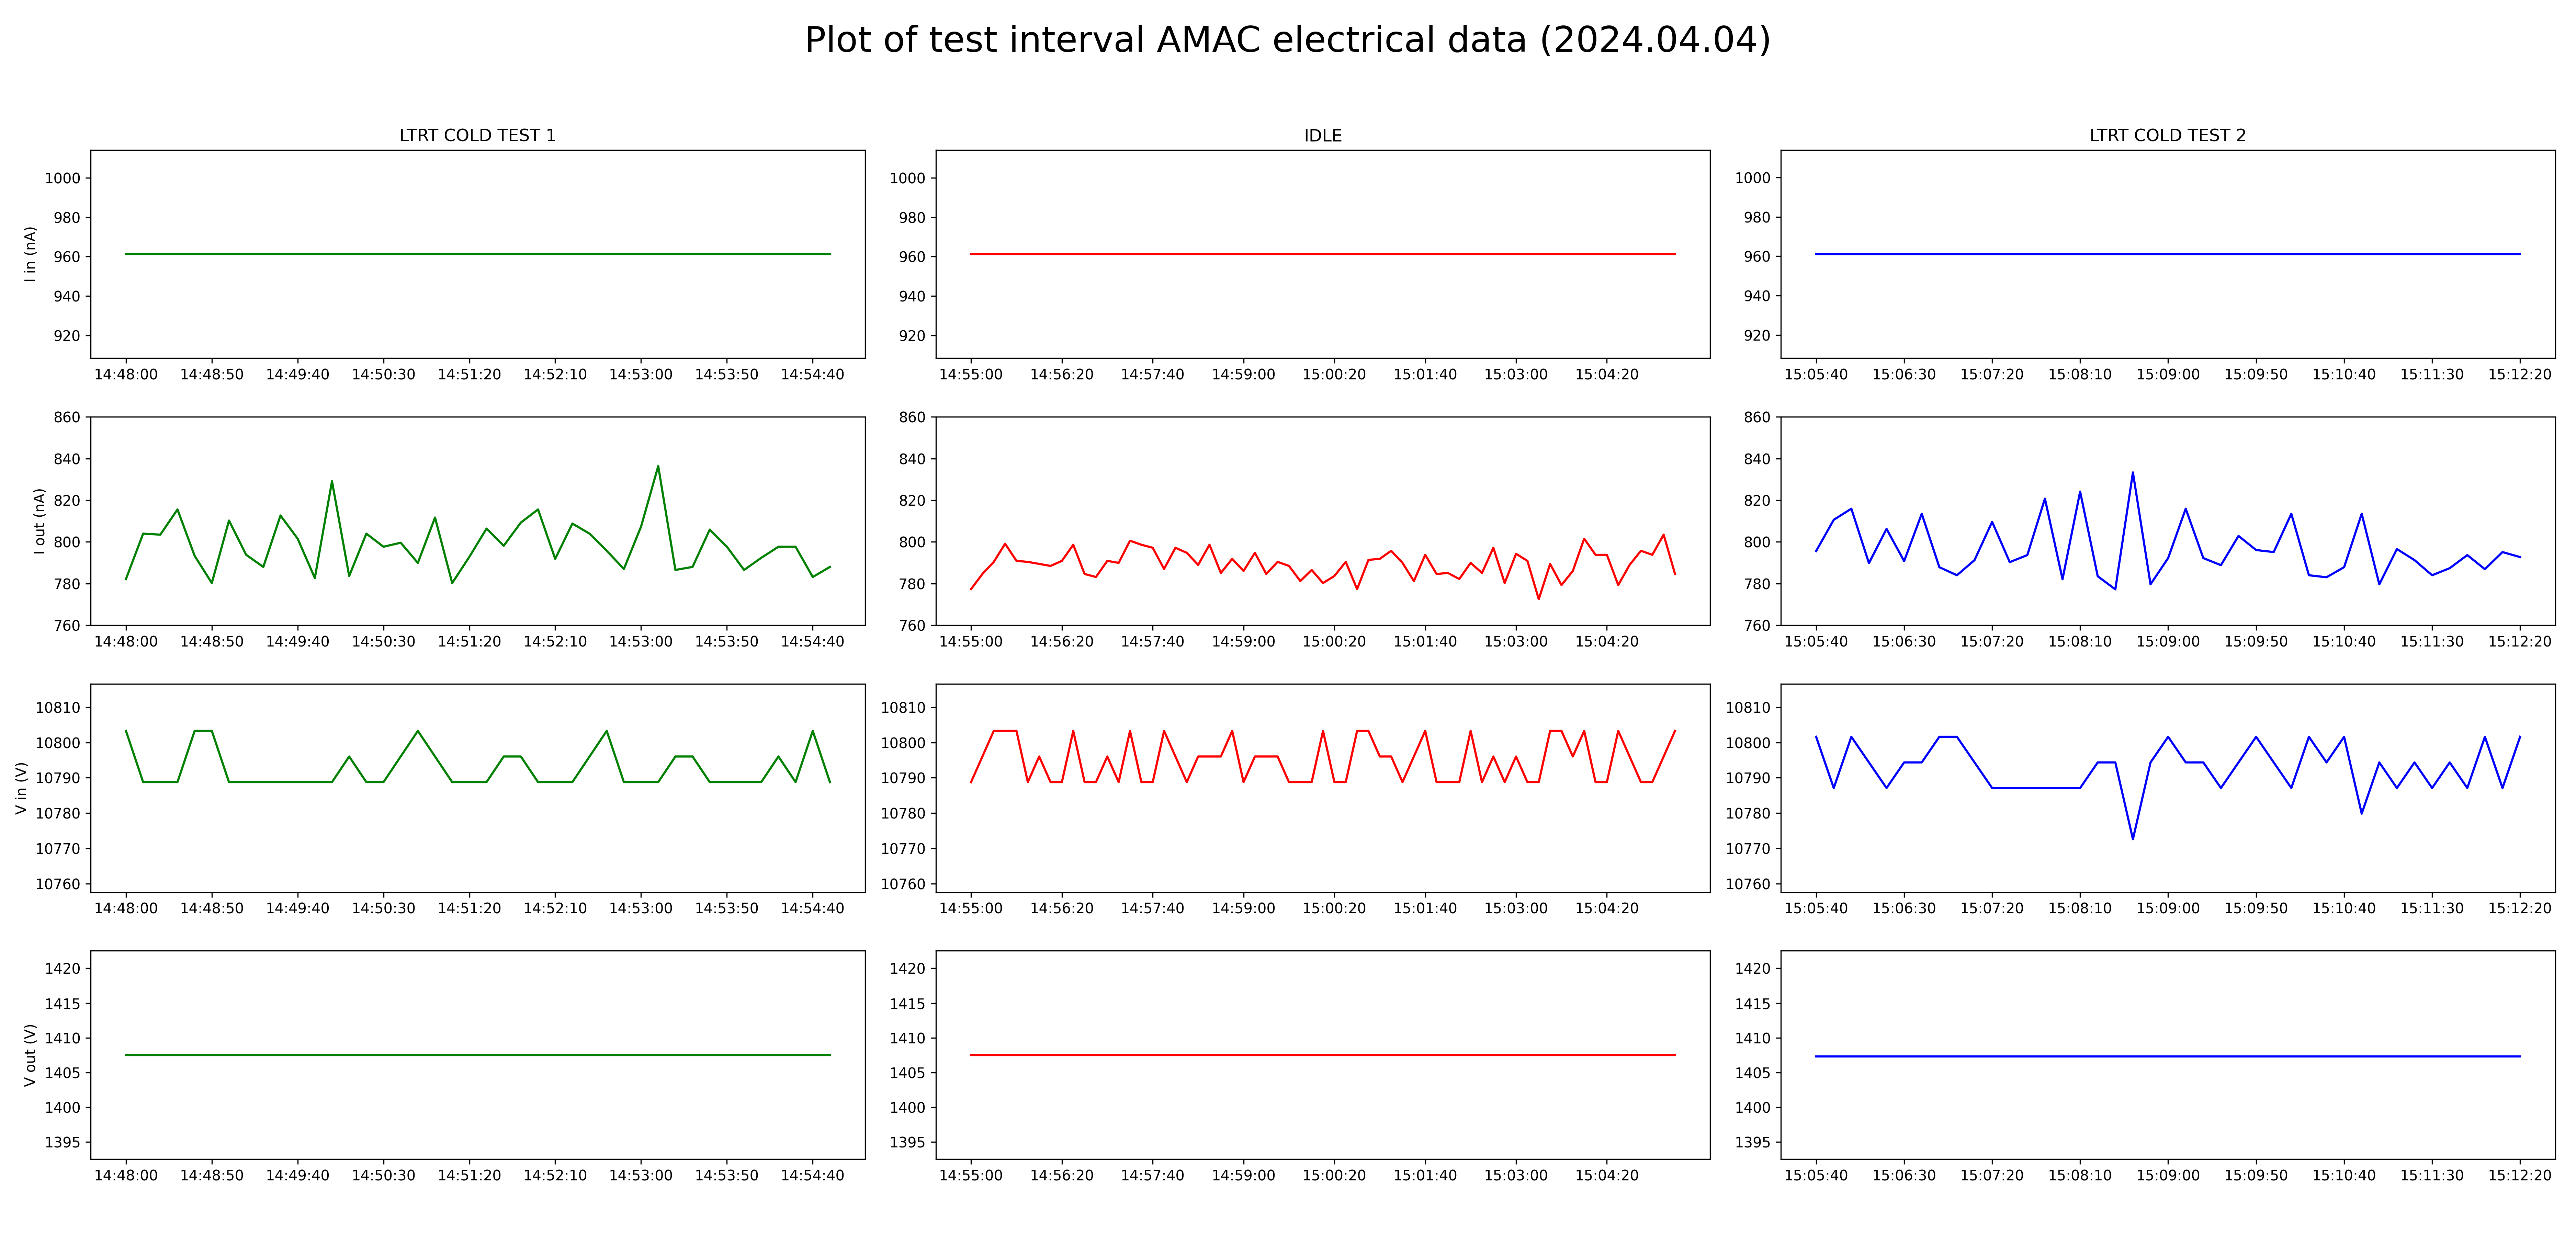
\includegraphics[width=25cm,height=20cm,keepaspectratio]{Figures/results/amac_el_plot_20240404_.png}
    \caption{Plots of AMAC electrical data showing the DC/DC input/output current (Iin/Iout), during the time span of the LTRT tests shown in Fig.\ref{fig:LTRT_result_1} and Fig.\ref{fig:LTRT_result_2}.}
    \label{fig:amac_el_large}
\end{sidewaysfigure}

\begin{sidewaysfigure}[h]
    \centering
    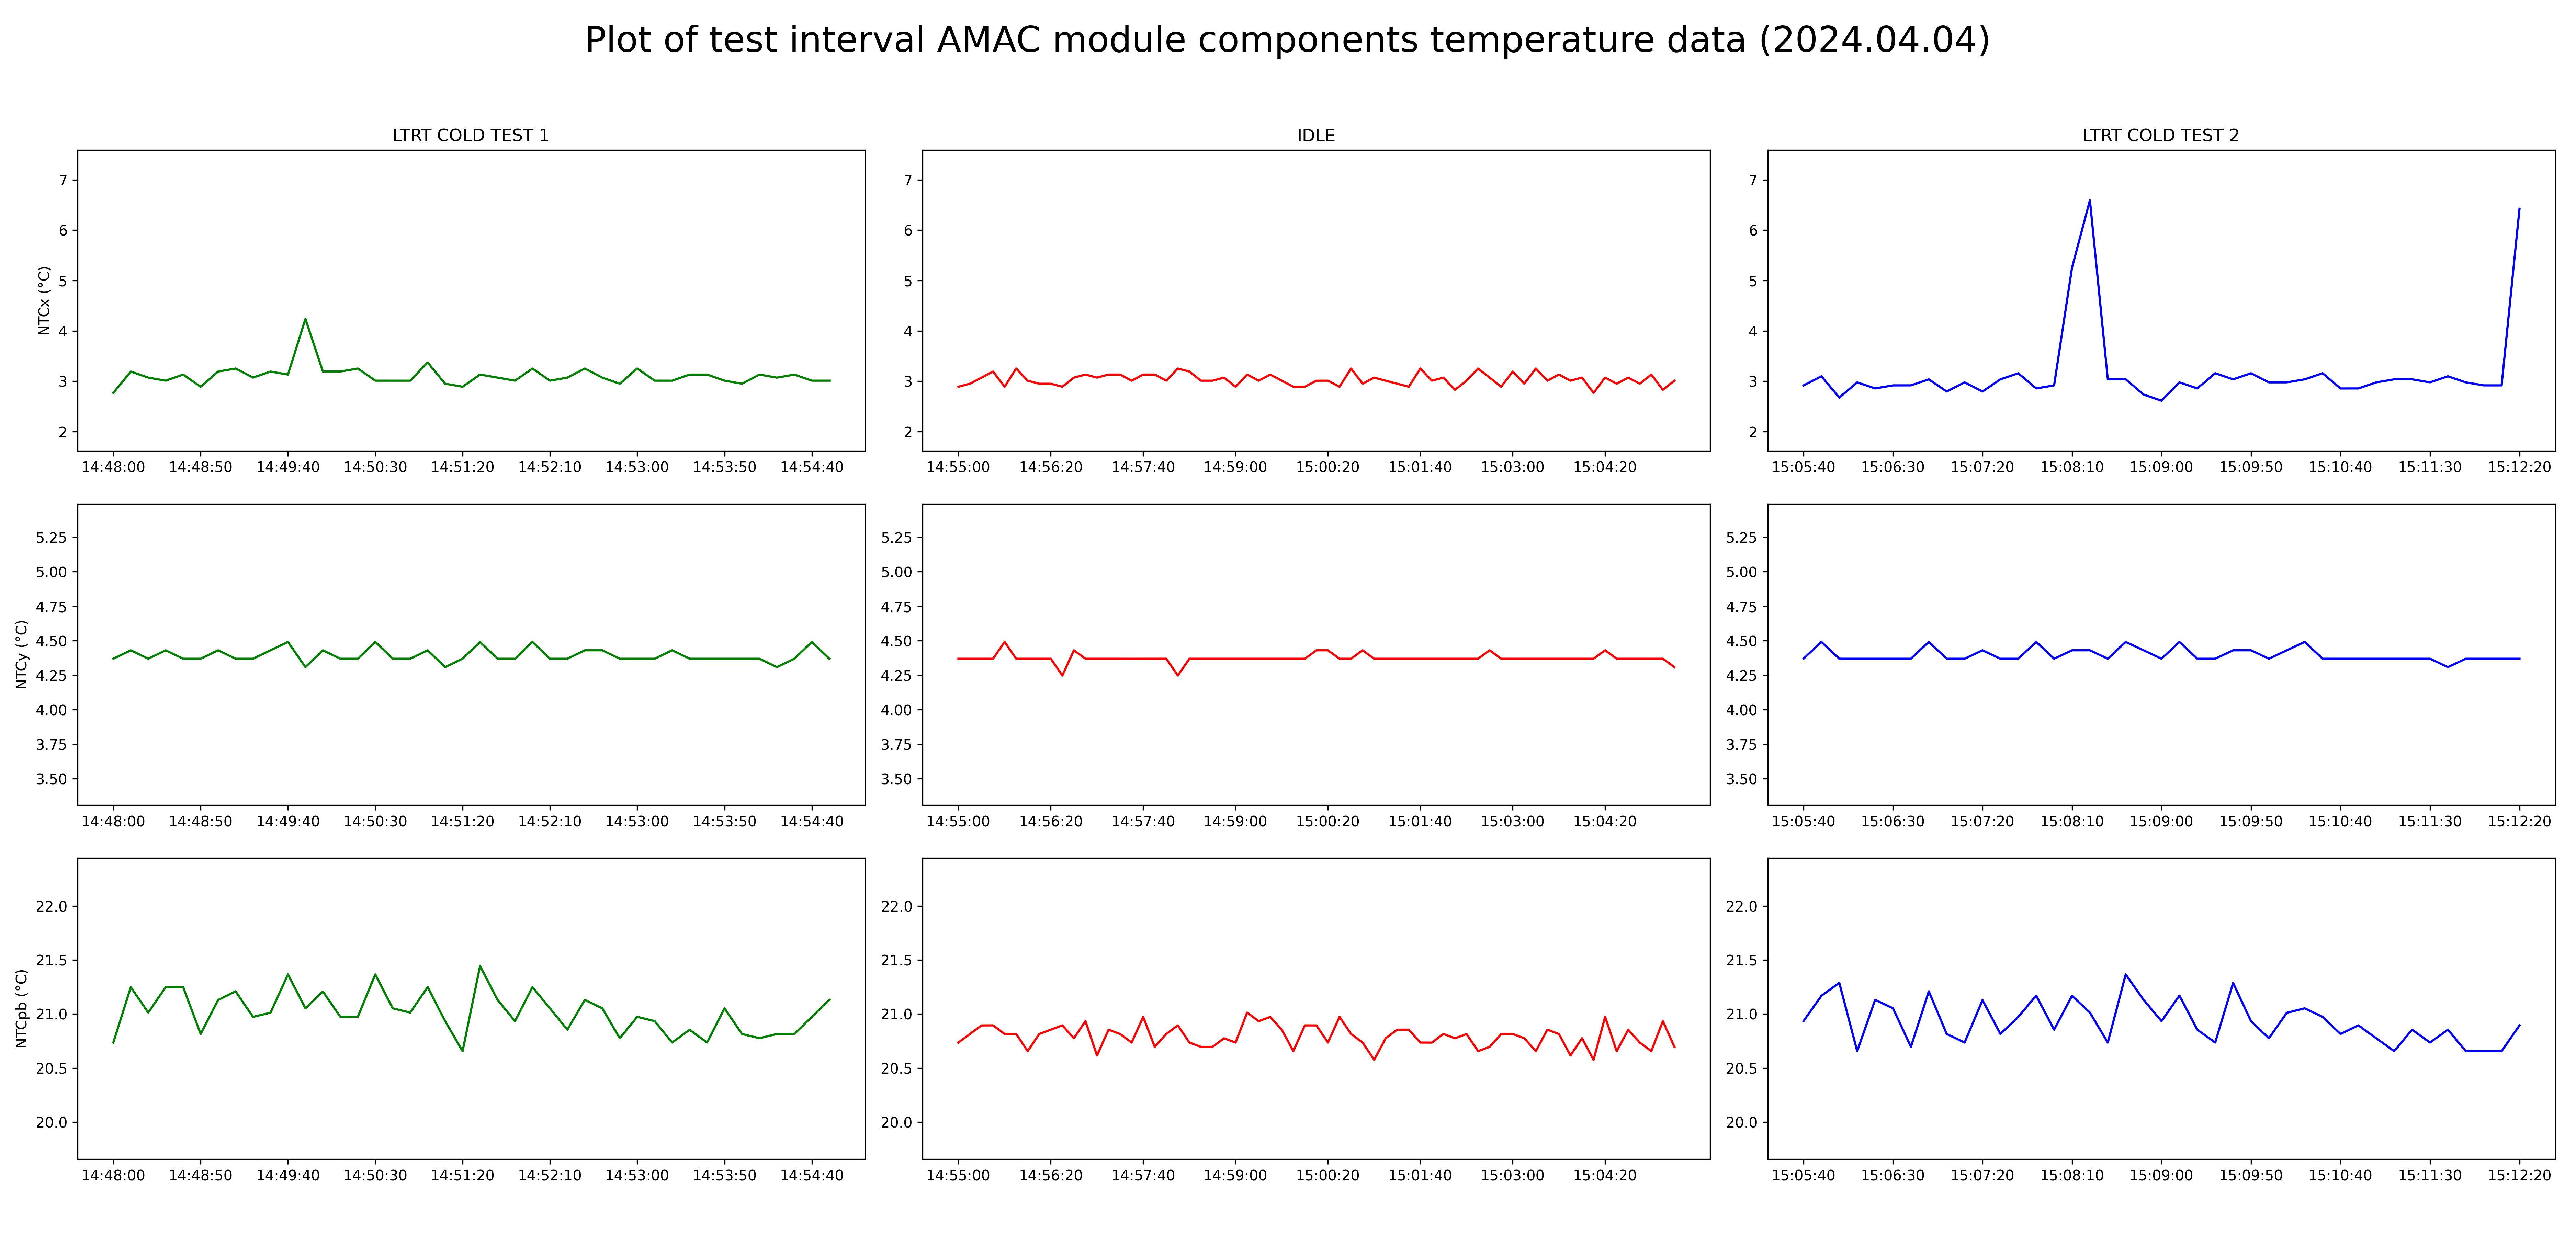
\includegraphics[width=25cm,height=20cm,keepaspectratio]{Figures/results/amac_temp_plot_20240404_.png}
    \caption{Plots of AMAC module components temperature showing the temperature on each of the hybrids (NTCx/NTCy) and powerboard (NTCpb), during the time span of the LTRT tests shown in Fig.\ref{fig:LTRT_result_1} and Fig.\ref{fig:LTRT_result_2}.}
    \label{fig:amac_temp_large}
\end{sidewaysfigure}